%!mode::"TeX:UTF-8"
\documentclass{ctexart}
\usepackage{amsmath}
\usepackage{amssymb}
\usepackage{xltxtra}
\usepackage{mflogo,texnames}
\usepackage{graphicx}
\usepackage{listings}
\usepackage{listing}
\usepackage{xcolor}
\usepackage{xcolor}
\usepackage{enumerate}
\usepackage[colorlinks,linkcolor=blue]{hyperref}
\usepackage{cite}
\usepackage{color}
\usepackage{caption}
\usepackage{subfigure}
\usepackage[top=2.54cm,bottom=2.54cm,left=3.18cm,right=3.18cm]{geometry}
\author{右武卫大将军}
\title{增强学习入门}
\begin{document}
    \maketitle
    \section{介绍}
        当我们在讨论什么是学习的本质时,第一个跳出来的念头就是我们是通过与环境交互来进行学习的。当一个婴儿在玩耍,抬起胳膊,或者四处观看的时候,他并没有一个明确的老师,但他确实通过一个传感器来与周围环境进行交互。通过这一传感器的连接可以产生关于原因与结果,动作之间的顺序,以及如何去做才能达成目标等很多有用的信息。纵贯人的一生,这样的交互无疑是人类获取环境知识和了解自身的主要方法。无论是驾驶汽车还是与他人谈话,我们都急切地想知道周围环境会针对我们的行为产生何种反应,也想通过自身的行为来影响可以发生的事件。从交互中进行学习是一切学习与智能科学理论的基本思想。

        本书所要探索的是用计算机的方式去从交互中进行学习。我们主要是探讨理想的学习环境和评估不同学习方法的效果,而不是去直接定义人或者动物是如何进行学习的。或者说,我们是从人工智能科学家或者工程师的角度来探讨这样一个问题。我们会探索一种能够有效解决科学研究或者经济活动中所面临的“学习”问题的一整套机制,并通过数学分析或者计算机试验的方式来评估这些解决机制。这里所要探讨的这一方法,被称为“增强学习”,相比于其他机器学习方法,它更加关注于目标指向性学习问题。
        \subsection{增强学习}
            增强学习是学习怎样做--即从环境映射到行动--来最大化数值化的奖励信号。学习器并不能告诉你哪一个行动是最优的,但是它可以通过测试来确定哪一个行动可以获得最大的奖励。在最有趣也最具有挑战性的情形下,行动可能不仅影响即刻的奖励也会影响下一刻的环境进而影响全部的后续奖励。这两种特点--试错搜索和延迟奖励--是增强学习两个最核心的特点。

            同很多用“ing”结尾的话题一样,比如机器学习(machine learning)或者登山运动(mountaineering),增强学习(Reinforcement Learning)同时指一类问题,一组解决问题的方案和研究解决问题方案的方法论。这三个问题使用同一个名称比较方便,但同时保持三个概念的独立性也是有必要的。特别的是,在增强学习中有效的区分问题和解决方案是很重要的,如果不能区分这两个概念会造成很多误解。

            我们用动态系统理论,尤其是基于马尔科夫决策过程的最优控制理论,来形式化描述增强学习问题。这一问题的详细描述要等到第三章的时候本书在讨论,不过其中的基本思想只是捕捉学习机器(Learning Agent)在不同时刻与环境交互来达成目标这一问题当中的主要方面。学习机器必须能够在某种程度上感知环境的状态,同时也可以采取行动来改变环境。学习机器必须根据环境的状态设定一个目标。马尔科夫决策过程主要将三个主要方面--感知,行动和目标--整合在最简单的形式当中,而不处理那些琐碎的部分。最适合解决这一类问题的方法,本书认为就是增强学习方法。

            增强学习不同于机器学习领域目前最广泛的有监督学习,有监督学习是从一组带标签的样本中进行学习,标签是由一个局外的监督者所提供的。每一个样本都有两部分构成,第一部分是环境的状态,第二部分是当前环境状态所对应的最佳行动,它也经常被视为当前环境状态所属的类别。这类学习的主要目标是解决从已有数据集上进行推断或者泛化来指导学习机器在未知环境中作出正确的行动。这是一种重要的学习方法,但是它很难解决从交互中进行学习的问题。在交互学习问题中,想要获取到既正确又能够涵盖学习机器可能遇到的各种环境状态下所需要采取的行动通常是不可行的。在未知的局面下,为了获取最大化的受益,学习机器必须能够从已有的经验中进行学习。

            强化学习通常也不同于机器学习研究者所说的无监督学习,无监督学习通常用于寻找无标签数据集中潜在的结构。从这个角度而言,监督学习和无监督学习似乎穷尽了各种各样的分类问题,但确实不是这样的。尽管很多人将增强学习视为无监督学习的一个分支,因为他并不依赖于带有正确行动标签的数据集,但增强学习是尝试最大化奖励信号,而不是探寻数据中的潜在结构。尽管探寻历史经验中的潜在结构在增强学习中有一定的作用,但是仅仅这一点是无法最大化奖励信号的。因此本书将增强学习认定为机器学习中与监督学习和无监督学习并列的第三种范式。

            增强学习中的一个在其他学习范式中不存在的问题是它需要解决\textbf{探索}(Exploration)和\textbf{压榨}(Exploitation)之间的折中问题。为了获取大量的奖励,增强学习机器不得不偏好于那些历史上它已经尝试过的,可以获得较多奖励的行动。但是为了发现这些\textbf{有效}的行动,增强学习机器又不得不去尝试之前他没有尝试过的行动。这就是说,增强学习机器既需要贪心地压榨历史上发生过的高奖励行动来确保高收益,但是它又不得不去尝试别的行动来测试是否存在更高收益的办法。这一矛盾的问题导致无论是过于贪心的压榨还是过于积极的探索都会导致任务失败。学习机器就不得不探索非常多的行动,同时又逐步偏向于那些看起来不错的行动。在一个随机任务中,每一个行动都需要被尝试很多次以获取对应奖励的可靠估计。探索和压榨的矛盾问题在过去的几十年中被广泛研究,目前也没有被完全解决。到目前为止,我们仅仅注意到,平衡压榨和探索的矛盾问题不存在于有监督问题或者无监督问题当中。

            增强学习的另一个重要特点是它需要在一个不确定的环境中考虑整个目标导向问题。相比之下,很多其他方法仅仅考虑的是子问题,而没有全局性的设想。比如,我们之前提过,很多机器学习研究关注于有监督学习,但是没有明确说明在实际应用中如何使用。其他研究人员进行过针对一般目标的理论,但是没有考虑在实时决策系统中如何应用。尽管这些方法得到了一些有用的结果,但是它们都关注于孤立的小问题而有很大的局限性。

            增强学习从一个完全的,交互的,目标指向性的问题开始,来解决相反的任务。所有的增强学习机器都是有明确的目标,可以感知环境的状态,也可以通过一些行动来改变环境的状态。而且,最开始就会假定增强学习机器所面临的环境具有高度的不确定性。当增强学习机指定计划时,它不得不考虑到计划和实时行动选择之间的交互以及环境模型是如何确定和改进的。当增强学习机涉及到有监督学习时,由于要决定哪一些能力是重要的,哪一些能力是不重要的,它就必须要这样做。为了学习研究能够取得进展,重要的子问题不得不孤立出来进行研究,但是它们同样是一个完整的,交互的,目标导向型的学习任务的一部分,即便整个学习问题的全部细节还不能完全搞清楚。

            一个完整的,互动的,目标导向的学习机并不总是意味着是一个完整的机器人或者有机体。 尽管它们是明显的例子,但是一个完整的,互动的,目标导向的学习机也可以是一个更大的行为系统的一个组成部分。 在这种情况下,学习机直接与较大系统的其余部分交互,并间接与较大系统所处的环境交互。 一个简单的例子是监控机器人电池充电水平并向机器人控制系统发送命令的学习机。 该学习机的环境是机器人的其余部分以及机器人所处的环境。 人们必须超越最明显的学习机及其环境的案例来理解强化学习框架的普遍性。

            现代增强学习最激动人心的一个方面是其与其他工程和科学学科的实质性和富有成效的交叉。增强学习是人工智能和机器学习数十年发展浪潮中的一部分,与统计学,优化和其他数学学科紧密结合。例如,一些增强学习方法用参数化逼近器的学习能力解决了运算研究和控制理论中经典的“维数灾难”问题。更有特色的是,强化学习也与心理学和神经科学强烈相互作用,双方都大有裨益。在所有形式的机器学习中,强化学习最接近人类和其他动物所做的学习,而强化学习的许多核心算法最初都受到生物学习系统的启发。通过动物学习的心理模型,更好地匹配一些经验数据,以及通过大脑奖励系统的相关研究,增强学习也有所改进。本书正文介绍了与工程学和人工智能相关的增强学习的思想,并在第14章和第15章中总结了与心理学和神经科学的联系。

            最后,增强学习是人工智能整个学科回归简单一般原则这一大浪潮中的一部分。从20世纪60年代后期以来,很多的人工智能研究学者认为,智能并没有一般性的方法,而是由大量的特殊的技巧,过程以及经验所构成。有时候会说,如果我们可以获取到大量的相关数据,比如数以百万或者十亿,塞进某台机器中,它就会变得很聪明。基于一般原则的方法,比如搜索或者学习,通常被称为“弱方法”,但是那些基于特定领域知识的的方法被称为“强方法”。这种观点现在还挺普遍,但是并不是唯一的看法。从我们的观点来看,这种观点是草率的,因为在研究一般方法的问题上还没有投入足够的努力所以不能够作出不存在这一类方法的结论。现代人工智能研究中有很多探求一般性方法的研究,目前还不清楚钟摆什么时间可能摆回来,不过增强学习是将人工智能推向简单,一般化原则和方法的重要力量。

        \subsection{例子}
            理解增强学习的一个好办法是了解一些曾经推动它发展的案例:
            \begin{itemize}
              \item 国际象棋下棋机是一个重要的进步。每一步棋都包括计划(即对手可能的回应)以及快速地,直觉性的对落子的判断。
              \item 自适应控制器实时调整炼油厂操作的参数。 控制器在指定的边际成本的基础上优化产量/成本/质量交易,而不严格遵守工程师最初建议的设定点。
              \item 一只瞪羚幼崽出生后几分钟就挣扎着。 半小时后,它以每小时20英里的速度运行。
              \item 移动机器人决定是否应该进入新房间以搜索更多垃圾来收集或开始尝试返回其电池充电站的路径。 它根据电池的当前充电水平以及过去回到充电器的历史经验来做出决定。
              \item 菲尔准备他的早餐。仔细检查,即使这个显然平凡的活动揭示了一个复杂的条件行为网和互锁的目标 - 子目标关系:走到橱柜,打开它,选择一个谷物盒,然后伸手去拿,抓住和取回盒子。需要其他复杂的,调整的,交互的行为序列来获得碗,勺子和牛奶盒。每个步骤都涉及一系列眼球运动,以获取信息并指导到达和运动。对于如何携带物品或者在获得其他物品之前将它们中的一些运送到餐桌上是否更好的快速判断。每个步骤都以目标为指导,例如抓勺子或到冰箱,并且服务于其他目标,例如一旦准备好谷物并且最终获得营养就吃勺子。无论他是否意识到这一点,菲尔都在获取有关他身体状况的信息,这些信息决定了他的营养需求,饥饿程度和食物偏好。
            \end{itemize}

            这些案例所共有的特征都比较简单,以至于很容易就被忽略了。全部都涉及到一个积极的决策机器和它所处的环境之间进行交互,尽管环境中充满了不确定性,但它还是努力去达成目标。机器的行动会影响到环境的未来状态(比如下一个国际象棋的位置,炼油厂的水库水位,机器人的下一个位置,以及它的电池电量),因此会影响未来的行动。正确的决策要求可以将这些非直接的,延迟的行动序列考虑进来,因此要求具有远见或者计划。

            同时,在这里例子当中,机器所作出的行动带来的影响不是完全确定的;因此机器就必须时时刻刻来监视其所处的环境。比如,Phil倒牛奶的时候必须要看着杯子中的状况以避免溢出。以上的例子都是有一个明确的,机器能够判断是否在向其逼近的目标。棋手当然知道其是否赢得了棋局;炼油厂控制器知道生产了多少石油,瞪羚幼崽知道它何时摔倒,移动机器人知道它的电池何时耗尽,菲尔知道他是否正在享用他的早餐。

            在以上的例子中,机器可以随着时间的增长利用之前的经验去改善它的性能,棋手可以提高他评估走棋的直觉,进而提高他的胜率;瞪羚的幼崽可以提高其跑动的效率;Phil学会了他制作早餐的标准流程。机器从最开始所携带的关于任务的知识--可能是来自于其他相似任务的经验,也有可能是设计机器时的预先设定--会影响机器学习何种知识,但是为了调整行为以探索任务的特定特征就需要机器与环境进行交互。

        \subsection{增强学习的元素}
            除了\textbf{机器}(Agent)和\textbf{环境}(Environment)之外,还可以在增强学习系统中确定出四个主要元素:\textbf{策略}(Policy),\textbf{奖励信号}(Reward Signal),\textbf{值方程}(Value Function),以及\textbf{环境模型}(Model of the Environment)。

            策略定义了学习机器在给定时刻上的行为方式。粗略来说,策略就是从一组环境的状态映射到所需要采取的行动的函数。它对应着心理学上的一个概念:刺激--回应法则。在有一些情况下,策略就是一个简单的映射方程或者查询表,但有些情况下,策略会涉及到进一步的比如搜索过程等额外的计算。策略是增强学习机器的核心因为它足以决定行动。一般来说,策略可能是带有随机性的,不同的概率采取不同的行动。

            奖励信号定义了增强学习问题的目标。在每一步中,环境告知增强学习机一个奖励值。学习机唯一的目标就是最大化它在整个流程中所获得到的奖励总和。因此奖励信号定义了什么事件对于学习机是好,什么事件是坏的。我们将奖励视为生物系统中的愉悦感或者疼痛感。它是学习机所面临的\textbf{即刻也明确}的核心问题。奖励信号是选择策略的主要基础;如果策略所选择的行动对应着低奖励,那么未来面对同样局面的时候策略就需要改进。一般来说,奖励信号是环境状态和采取行动的随机函数。

            奖励信号指示了在当前时刻什么是好的,而值方程说明了在长期过程中什么是好的。粗略地说,某一个状态的\textbf{值}(Value)是学习机从当前状况开始未来所可能获取到的奖励总和。奖励信号决定的是当前状况即刻的,重要的评分,而值指示了在考虑到未来可能的状态以及伴随这些状态可能的奖励的基础上对当前状况的长期评分。比如说,一个状态可能在眼下奖励很低,但是它对应的值却很高,因为该状态所引出的后续状态的奖励很高。或者是相反的情况。从人的角度而言,奖励在某种程度上就是愉悦感(如果高的话)或者疼痛感(如果低的话),而值对应着从长远角度来看我们当前所处的状态对一生造成的愉悦感或者痛苦感。

            可以这样说,奖励是即刻的反馈,是最重要的指标,而值作为对奖励的预测是第二重要的指标。没有奖励的话就没有值,而估计值的唯一目的是为了获取更多的奖励。尽管如此,我们在进行决策时仍然将值作为首要考虑目标。基于值的判断来做出行动的决策。我们寻求能够带来最大值的状态以及通往该状态的行动,这样的行动可以保证我们在长期中获得最大的受益。但不幸的是,得到状态对应的值的难度要远远高于得到状态对应的奖励。奖励一般可以直接由环境所给出,但是值的估计需要基于整个流程中的一系列状态观测。实际上,在几乎所有的增强学习问题中最重要的问题就是寻找一种高效的评估值的方法。这一问题是在之前六十年的增强学习研究中最中心的问题。

            第四个也是最后一个增强学习系统的模块是关于环境的模型。这个模型在某种程度上就是对环境行为的模拟,或者,更一般而言,它可以对环境可能做出的反映做出预测。比如,给定环境的状态和学习机采取的行动,该模型可以预测出环境的下一个状态和对应的奖励。模型可以辅助计划,通过计划我们可以在未来局面尚未出现的情况下对奖励进行估计。利用模型和计划来解决增强学习问题的方法被称为基于模型的方法,与之相对应的是无模型方法,也就是通过试错的办法来寻求最优方案,这几乎是计划的反义词。在第八章我们会讨论通过试错法进行调整的增强学习系统。现代增强学习系统有很多的变种,从很简单的试错式的学习到很复杂的模型式学习。

        \subsection{局限性和展望}
            增强学习很依赖于状态的概念--状态是策略和值方程的输入值,同样也是环境模型的输入和输出。简单来说,状态就是一个信号,告诉学习机在某一时刻环境是什么样子的。正式关于状态的定义会在第三章讨论马尔科夫决策过程框架时提出。不过,本书还是鼓励读者按照非正式定义去理解状态这一概念,也就是学习机能够感知到的全部环境状态。实际上,我们假定状态信号是由很多构成环境系统的进程来产生的。当然在本书中我们并不讨论状态信号的构成,改变或者学习之类的问题。我们这样做的原因不是因为状态的产生原因不重要,而是说把注意力集中于决策生成系统中。换言之,本书的研究核心不在于设计状态信号,而在于无论何种状态信号出现都能够做出恰当的行动。

            本书中所讨论的大多数增强学习算法都是围绕着如何构建值方程这一问题的,但是这并不是解决增强学习问题的必须方法。比如,诸如生成式算法,生成式编程,模拟退火,以及其他最优化算法等Solutions类方法并不需要估计值函数。这些方法应用多个静态策略,每个策略在较长时间内单独的与环境进行交互。 获得最多奖励的策略及其随机变化将延续到下一代策略,并重复该过程。 我们称之为这些进化方法,因为它们的操作类似于生物进化产生具有熟练行为的生物的方式,即使它们在个体生命期间不学习。如果策略空间足够的小,或者说可以被结构化的表述,以至于好的策略是很容易被发现的,那么进化类算法的效率是比较高的。此外,进化类方法在学习机不能感知到环境的全部状态时也很有优势。

            本书所探讨的增强学习算法是那种与环境相交互的,通常进化类算法并不考虑这一点。在很多情况下能够利用个体行为之间的交互的方法通常比进化类方法更加有效,进化类方法忽略了增强学习问题中很多有效的结构:它们没有利用要搜索的策略是一种从状态到行动的映射;它们没有关注个体在整个流程中会经历那些状态或者说选择哪些行动。在有些情况下,这些信息具有误导性(比如,某个状态是错误记录的数据),但在更多情况下,这些信息可以提高效率。尽管进化算法和学习算法有很多共同点并且也相互协作,但本书并不认为进行算法适合解决增强学习问题,因此,我们在本书中并不讨论这种算法。

        \subsection{详细的案例:Tic-Tac-Toe}
            为了说明增强学习的一般思想,并将其与其他类型的方法相对比,我们接下来详细讨论一个简单的例子。

            考虑一个熟悉的儿童游戏:Tic-Tac-Toe。两位棋手在一个三乘三的格子上轮流下棋。一个棋手执X,一个棋手执O,轮流下棋,直到一个棋手的三个棋子连成一行,横的,竖的,或者对角线的。如果棋盘下满了也没有一个棋手取得胜利,那就是平局。因为一个有经验的棋手可以确保自己一定会赢,所以我们假设对手没那么多经验,会走很多错误的棋。另外,我们假设平局和失败对我们来说是没有区别的。那么我们怎么样才能构建一个智能机器来充分利用对手的纰漏来提高自身的胜率呢?

            尽管这是一个简单的问题,但是使用传统的方法还是很难解决的。比如,传统的游戏理论中的“极大化极小(minimax)”方法在这里并不正确,因为这种方法必须假设对手以某种特定的方式来走棋。比如,Minimax棋手永远都不会走到一个可能会输的位置上去,即使说因为对手的纰漏,他走到那里也是可以赢得比赛的。传统的针对序列决策问题的最优化方法,比如动态决策过程,会计算对手的最优应对方式,但这需要获得对手的完全信息,包括在每一个棋面之下对手走不同的棋子的具体概率。我们这里假设没有这些先验信息,因为它不适用于大多数我们想要研究的问题。另一方面这一部分信息可以通过与对手多次博弈来进行估计。解决这一问题最佳的方法是首先学习一个关于对手行为的模型,达到一定的置信水平之后,使用动态规划的方法来计算最优的策略。最后,这与我们后面在本书中讨论的一些增强学习方法不同。

            应用于该问题之上的进化类算法会直接探索可行的策略空间以寻求一个具有较高获胜概率的策略点。这里的策略点指的是一个函数,可以从任何可能的棋盘状态上映射出一种走子的决策。对于任何一种待考虑的策略,其获取的概率都可以通过多次和对手下棋来进行估计。这种评估方法可以指导下一轮次应该考虑哪一种策略。一个典型的进化类方法会在策略空间内使用爬山策略,紧接着会生成和评估策略以获得明显的改善。或者说,可以获取并评估整个策略空间的生成式方法可能是适用的,论文中有数百种不同的优化方法可以使用。

            接下来我们讨论利用值方程的方法来解决Tic-Tac-Toe问题。首先我们设定一个数值表,每一个数值对应着游戏中的一个状态。这个数值代表的是从该状态开始能够赢得比赛的概率的最后一次估计值。换言之,这个数值就是该状态对应的“值”,而整张表就是所谓的“值方程”。状态A的值大于状态B的值就指的是从状态A开始获得胜利的概率要远大于状态B。假设我们一直执X,那么那些三个X子排成一行的状态获胜的概率就是1。相似的,如果三个O子排成一行,或者棋盘下满子,那么获胜的概率就是0。我们将其他棋盘状态的初始值都设定为0.5,代表从目前的状态开始有50\%的概率获取胜利。

            \begin{figure}
                \centering
                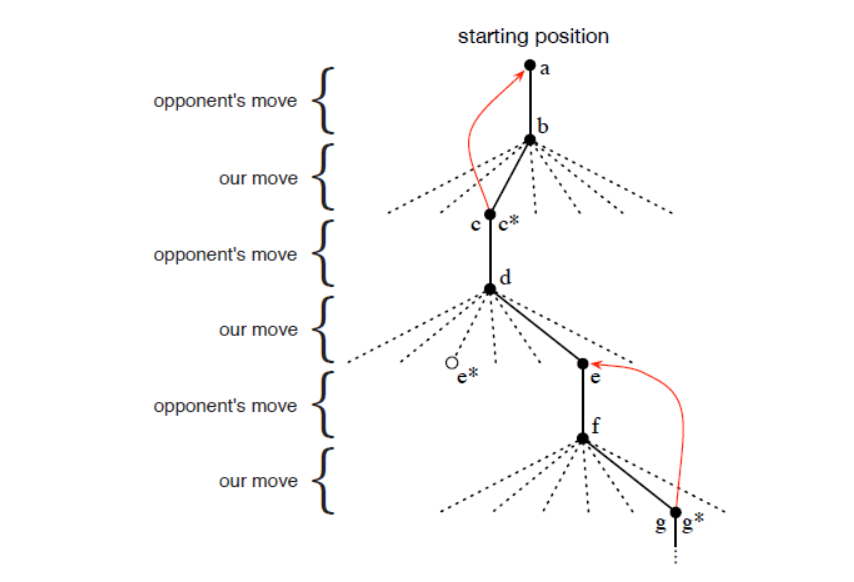
\includegraphics[width=0.8\textwidth]{f1-1}
                \caption{Tic-Tac-Toe游戏的走子序列。黑色实线代表游戏中的实际走子;虚线代表候选的走子方案。而第二步我们执行的是探索走子,也就是说存在一个走子方案$e^*$的值更高。探索性走子不会促使任何学习行为的产生,但是后续的走子可以辅助值方程的更新,如图中红色箭头所示}
                \label{f1_1}
            \end{figure}

            我们会和对手反复进行游戏。为了决定走哪一步,我们对比可能的走子位置所形成的棋面状态,并根据值方程表中其对应的值。大多数情况我们会比较“贪心”的选择可以达成最大胜率的那个状态。但是有些时候也会随机选择其他的走子方式。这种走子我们通常称为探索行为,因为这样可以帮助我们尝试之前没有出现过的状态。整个的走子序列可以概括为图\ref{f1_1}所示。

            在反复下棋的过程中,我们就可以更新每一个状态所对应的值,对胜率的估计越来越准确。为了实现这一点,在每一步贪心走子之后我们都需要回溯到之前的状态,如图\ref{f1_1}中红色箭头所示。更精确的说,早期状态的值会被更新到更接近于后期状态点的值。通过按照一定比例将后期状态的值合并到早期状态的值中可以达成这一点。记$S_t$代表贪心走子之前的状态,而$S_{t+1}$代表走子之后的状态,而状态$S_t$对应的估计“值”$V(S_t)$在更新之后的新值如下式所示:
            \begin{equation}
                V(S_t) \rightarrow V(S_t) + \alpha [V(S_{t+1})] = (1-\alpha)V(S_t) + \alpha V(S_{t+1})
                \label{e_1}
            \end{equation}
            其中$\alpha$是一个比较小的正比例系数,被称之为步长参数,会影响到学习的速率。这一更新方法是时序差分学习方法的一个例子,之所以起这样的名字,是因为它的更新是基于两个相邻状态的值差分$V(S_{t+1}-S_{t})$的。

            在当前的任务中上述方法非常的有效。比如说,如果步长参数随着时间的增长逐步降低,那么给定不变的对手,上述方法就会收敛到当我们按照最优走子方案所能达成的胜率。更进一步而言,除去那些探索性走子,我们所选择的走子就是针对对手的最优走子方案。换言之,这个方法就可以逼近到下棋的最优策略之上。另外,即使对手在改变自己的下棋风格,但只要变化的速度不快,那么只要步长参数不退化为零,上述方法也是有效的。

            这个例子说明了进化类算法和基于值方程的方法的区别。为了评估一个策略,进化类算法会保持一个策略固定,然后不停地与对手下棋,或者是模拟对手进行下棋。获胜的频率给出了获胜概率的无偏估计,进而可以直接指导策略的选择。但是每一次更新策略都需要进行大量的棋盘测试,并且每一盘棋只有最终结果被加以利用,而在下棋的过程中的事件是毫无用途的。比如,棋手获胜之后,它所下的每一步棋都被认为是合理的,而忽视了中间过程中哪一些走子是特别重要的。甚至来说,合理性都被赋予给了那些从来未在棋盘上出现的走子方案。相对比而言,值方程方法可以对每一个棋盘状态进行评估。最后,进化类算法和值方程算法都在探索整个策略空间,但是对值方程进行学习的过程可以充分利用整个棋局可以加以利用的信息。

            这一个简单的例子展现了很多增强学习方法的关键特征。首先,在这个案例中强调了利用与环境的交互进行学习,这里的环境就是对手的策略。其次,这个案例有一个明确的目标,而且要求能够充分考虑决策的滞后影响。比如一个简单的增强学习机可以通过设置一个小陷阱来诱骗短视的对手。增强学习解决方案一个特别吸引人的优点是,它无需利用环境的模型也无需给出明确的未来可能出现的状态和行动就可以达成极具远见的策略。

            尽管这个例子展现了增强学习的一些核心特点,但是它过于简单以至于大家会忽视增强学习的巨大潜力。尽管Tic-Tac-Toe是一种两人游戏,但增强学习是可以推广到不存在明确外部对手的情况上的,或者说是与“大自然进行对抗”。同样增强学习也不仅仅局限于这种行动被切分为标准回合的特定类型任务,或者是奖励只有在最后一刻才出现的任务。它在那种有无限次决策机会或者奖励在任意时刻出现的任务上也是适用的。增强学习同样适用于非离散决策的任务。连续性任务通常会复杂一些,在入门介绍阶段我们就暂时不再涉及。

            Tic-Tac-Toe游戏有一个相对较小的,有限的状态集合,但增强学习通常也适用于状态空间非常巨大的情况。比如,Gerry Tesauro(1992,1995)将上述方法和人工神经网络相结合来对国际象棋进行学习,而国际象棋的状态空间大约为$10^{20}$这样的规模。因为状态空间极其庞大,遍历其中很小的一部分都是极其困难的。Tesauro的程序最终超过了之前的模拟程序,并最终战胜了国际象棋冠军。人工神经网络提供一种可以从经验中进行泛化的能力,所以当它面临相似的局面的时候可以做出类似的决策。增强学习在这样庞大的状态空间中学习的好坏与否取决于它能多好的从历史经验中进行推广泛化。所以我们不得不在增强学习中混入有监督学习,不过人工神经网络或者深度学习并不是唯一的选择。

            在Tic-Tac-Toe游戏中,除了游戏的规则之外并没有其他的先验知识,不过通常增强学习需要有先验知识。先验信息有很多方式可以将其整合到增强学习当中,这些方式会对增强学习的训练产生重大影响。在Tic-Tac-Toe游戏中,所有的游戏状态都是显性的,但在很多增强学习案例中环境的状态都是隐性的,或者说不同的状态从外部看起来是一样的。

            最后,Tic-Tac-Toe游戏每一步的走子和走子所达成的状态是严格对应的,可以被预先知道。如果在实际增强学习应用中做到这一点,那就需要对环境进行建模,基于该模型就可以指定每一个动作所对应的状态,即使该行动从来没有出现过。很多问题都存在这一问题,但是还有一些问题仅仅建立行动的短期影响都是很困难的。不过在这两种情况下增强学习都是可以应用的。关于环境的模型不是必须的,但是如果有这样的模型也可以很容易的融入到增强学习中。

            另一方面,有一些增强学习算法是完全不需要关于环境的模型的。无环境模型系统甚至都不需要考虑学习机的每一个行动对环境的影响。Tic-Tac-Toe的游戏玩家在这种意义上就是无环境模型的,即对对手的行为是不预测的。之所以有不利用环境模型的系统是因为如果想让环境模型系统产生一定的效果,就需要环境模型能够达到足够的精度,但在很多情况下,这是做不到的。无环境模型系统是有环境模型系统的基础。本书我们会首先讨论无环境模型系统,然后以此为基础讨论有环境模型系统。

            增强学习既可以作为一个高层级系统,也可以作为一个低层级系统。尽管在上述游戏中,增强学习用以学习每一步棋如何走,但增强学习也可以用于学习一套解决方案,即每一方案就是解决问题的全套步骤。在层次学习系统中,增强学习可以同时在多个层级上工作。

        \subsection{总结}
            增强学习是一种有利于理解目标性导向学习和决策的计算方法。它与其他类型计算方法的主要区别就在于它强调学习机与环境的直接交互,而不需要一个明确的监督者或者关于环境的模型。在本书看来,增强学习方法是第一种能够处理与环境交互来达成长期目标的人工智能方法。

            增强学习使用状态,行动,奖励,值方程等一系列概念来刻画学习机和环境之间的交互,并利用正式的马尔科夫决策过程来进行学习。这种架构尝试使用一种简单的方法来对人工智能所涉及的必要元素进行表示。这些元素包括因果联系,不确定性和明确的目标。

            值和值方程的概念是大多数增强学习方法的核心概念。我们认为值方程是提高策略空间搜索速度的有效方法。值方程是区分增强学习方法和进化类方法的主要特征,进化类方法遍历性的探索整个策略空间。

    \section{多臂老虎机游戏}
        这一章以及后续几章,本书会以各自最简单的形式介绍增强学习算法的全部核心概念:状态空间和行动空间会特别的小,保证值方程可以以表格的形式来呈现。在这种情况下,增强学习方法通常可以找到最优的值方程和最优的策略。与本书另一部分将介绍的近似方法相比,近似方法只能发现近似解,不过近似方法在大型问题上的效率比较高。

        这一部分的第一章会首先介绍增强学习的一个特殊案例:只有一个状态的环境,被称为赌博机问题。第二章会介绍一个一般的问题范式,也是本书主要讨论的问题,有限马尔科夫决策过程,这其中涉及到的主要思想是Bellman方程和值方程。

        后面的三章就会刻画三种解决有限马尔科夫决策过程的基础性方法:动态规划,蒙特卡洛方法以及时序差分学习。每一种方法都有它的优点和缺点。动态规划算法在数学上非常严谨,但是它需要知道精确的环境模型。蒙特卡洛方法不需要知道模型,计算上也很简单,但不太适用于轮次决策的问题,最后时序差分方法不需要知道环境模型,也适用于轮次决策过程,但是在分析上非常的复杂。这些方法在效率和收敛速度上也有所不同。

        最后的两章会介绍如何将这三种方法结合起来以充分利用各自的优点。前面一章我们介绍如何将蒙特卡洛方法的优点和时序差分方法的优点,通过多步的BootStrapping方法结合起来。而后面的一章时序差分方法如何与诸如动态规划等模型类方法结合,构建一个完备的,统一的增强学习问题解决方案。

        区分增强学习和其他类型学习的核心特征是它利用训练过程中的信息去评估行动而不是给定正确的行动来指导学习。正是这一特点要求增强学习需要进行探索性行动以寻求效果更好的行动。单纯的评估性反馈仅仅指示了行动的绝对得分,而并不能指明它是不是最好或者最坏的行动。另一方面,单纯的指示性反馈独立于实际采取的行动,可以指明应该采取的正确行动是什么。这种反馈是有监督学习的基础。在其纯粹形式中,有两种不同的反馈:依赖于实际采取行动的评估性反馈,独立于实际行动的指示性反馈。

        本章中以一种简单的方式来研究增强学习的评估方面,所谓的简单就是状态空间只有一个值。这种非结合式的设定其实就是说涉及到评估式反馈的大部分先验性信息都已经获取到了,也就避免了完整的增强学习方法中很多复杂的内容。研究这一案例,可以帮助我们更清晰的了解评估性反馈和指导性反馈的区别,以及如何将两者相结合。

        本章所探索的这一特定的,非结合式的评估性反馈问题是多臂赌博机问题的一个简单版本。借助于该问题会引入很多基础的学习方法,这些方法会在之后的章节被拓展以适用于更加全面的增强学习问题当中。在本章的最后,会通过假定如果多臂赌博机是结合式的,也就是说状态空间很有很多状态来构成,那么本章讨论的问题就会转变为一个标准的增强学习问题。

        \subsection{多臂赌博机问题}
            考虑以下的学习问题。你需要反复的在$k$个不同的选项中作出抉择。每一次决策之后,你就会得到一定量的奖励,具体的量是从一个你的决策所对应的固定的分布中所获取的。你的目标是最大化在多轮决策中获得最大量的奖励。

            这是多臂老虎机问题的初始形式,之所以这么叫是因为它通过一个投硬币的赌博机来形象的刻画。每一次决策都类似于拉下赌博机上的某一个拉杆,而奖励就是中奖后赌博机吐出的硬币。尽管会进行多次决策,但为了获得最大利益,你只会拉那个收益率最高的拉杆。另一个类似的例子是医生会在多个试验性的疗法中进行选择以应用多个病人身上,每一次决策都是在病人身上使用哪一种疗法,而奖励就是病人的存活率。其实实际应用中有很多类似的推广应用,但是本书就仅仅研究这一个简单的问题。

            在多臂赌博机问题中,在给定所选决策之后,每一个决策都对应着一个期望收益,我们将期望收益称之为决策的“值”。记在第$t$时间步的决策为$A_t$,对应的奖励为$R_t$。某一决策$a$的值记为$q_{*}(a)$,是决策$a$对应的期望收益:
            \begin{equation}
                q_{*}(a)\dot{=}\mathbb{E}[R_t|A_t=a]
                \label{e_2}
            \end{equation}
            如果可以知道每一个决策对应的值,那么多臂老虎机问题就变得很简单了,直接选择值最大的决策就可以了。我们把这种决策称之为贪心决策,或者贪心行动。如果你基于当前的值方程,作出选择值最大的行动,我们把这种选择称为压榨已有信息。反之,如果你选择某一个非贪心的决策,我们称之为探索新的信息,因为这样的行为可以更新对应行动的值。压榨行为在一次行动中可以获得最大的受益,但探索行为可以促使在长期中获得较高的总受益。比如说有一个“占优”决策的值是确定的,还有几个其他决策被估计和“占优”决策的值差不多大,但是不确定,这种不确定指的是这几个决策中至少有一个是优于目前的“占优”决策的,但是是哪一个并不知道。如果你有很多的决策机会,那么进行这种探索行为,确定哪一个行动比当前的“占优”决策更好是有利的。探索行为在短期内是一种较差的行为,而在长期中是一种较好的行为,因为你可以发现新的“占优”决策,并在未来继续压榨它。由于不能在一次决策中同时进行“压榨”和“探索”,所以行为人就不得不在这两个选项上进行平衡。

            在具体问题上,“压榨”或者“探索”哪一个更好,取决于当前值方程的精确度,环境的不确定性,以及剩余的决策步数。基于具体的多臂赌博机或者其他类似问题的数学方程,有很多复杂的方法可以在探索和压榨之间进行平衡。但是,这些方法中的大部分要求对先验信息或者环境的稳定性作出很强的假设,这在实际应用或者标准的增强学习问题中是很难达成的。这些方法在以上假设不成立的时候其最优性或者损失界是不能保证的。

            本书中,我们并不担心平衡压榨和探索过于复杂,只担心是不是能够平衡。本章会就多臂赌博机问题提出几种简单的平衡方法,并证明这种方法要比一直压榨的效果好一些。需要平衡探索和压榨是增强学习的一个独有的特色,本章的简化多臂赌博机问题可以很清晰的展现这一点。

        \subsection{动作-值(Action-Value)方法}
            首先我们先探讨估计行动的值的方法以及使用这个估计结果来做出行动决策,我们把这样整个流程称为\textbf{行动-值}方法(Action-Value Method)。所谓行动的值就是采取该行动所获得的平均奖励,最自然的方法就是在实际测试结果上做平均。
            \begin{equation}
                Q_t(a) \dot{=} \frac{\sum_{i=1}^{t-1}R_i \cdot \mathbb{I}_{A_i=a}}{\sum_{i=1}^{t-1}\mathbb{I}_{A_i=a}}
                \label{e_3}
            \end{equation}
            其中$\mathbb{I}_{predicate}$是指示函数,当下缀的判断语句为真时,指示函数值为1,而当下缀的判断语句为假时,指示函数值为0。如果上式中分母为0,那么我们就将$Q_t(a)$定义为默认值,比如0。当分母的值无限大时,根据大数定律,$Q_t(a)$会收敛到$q_{*}(a)$。我们将其称为估计值方程的样本平均法,因为每一个行动对应的值实际上就是历史回报的平均值。当然该方法只是其中一种方法,也不一定是最优的方法。不过暂时我们假定只有这一种方法,并基于该方法来讨论如何基于值方程作出决策。

            最简单的决策原则就是选择当前值方程中值最大所对应的行动,也就是前期行动结果所应当的最贪心的行动。如果有两个行动的值是相同的,那么就可以用随机的办法来决定选择哪一个。我们形式化的将这种贪心策略记为:
            \begin{equation}
                A_t \dot{=} \operatorname*{argmax}\limits_{a} Q_t(a)
                \label{e_4}
            \end{equation}
            贪心策略总是利用历史知识最大化眼前的利益,它不依赖于时序上的信息就可以从历史信息中提取到最优的行动。一种简单的备选方案是大多数时刻都进行贪心行动,而在很小的概率$\epsilon$下,随机的等概率的选择其他行动,而不参考行动值方程的估计结果。我们将这种极其接近贪心方案的方法称为$\epsilon$-贪心方法。该方法的优点是,如果进行决策的次数是无限多次的,那么每一个行动也会被尝试无限多次,这就确保了$Q_t(a)$会收敛到了$q_*(a)$。这一方法中选择当前最优的策略的概率是大于$1-\epsilon$的,接近于确定。但是,以上所说的收敛也只是渐近式的,其实际效率没有保证。

        \subsection{10臂赌博机测试}

            为了大致评估贪心方法和$\epsilon$- 贪心方法的相对效率,我们在一系列的问题上对其进行数值上的对比。测试数据是由两千次10臂赌博机随机产生的结果,图\ref{f2_1}展示了不同的拉杆对应的回报分布。
            \begin{figure}
                \centering
                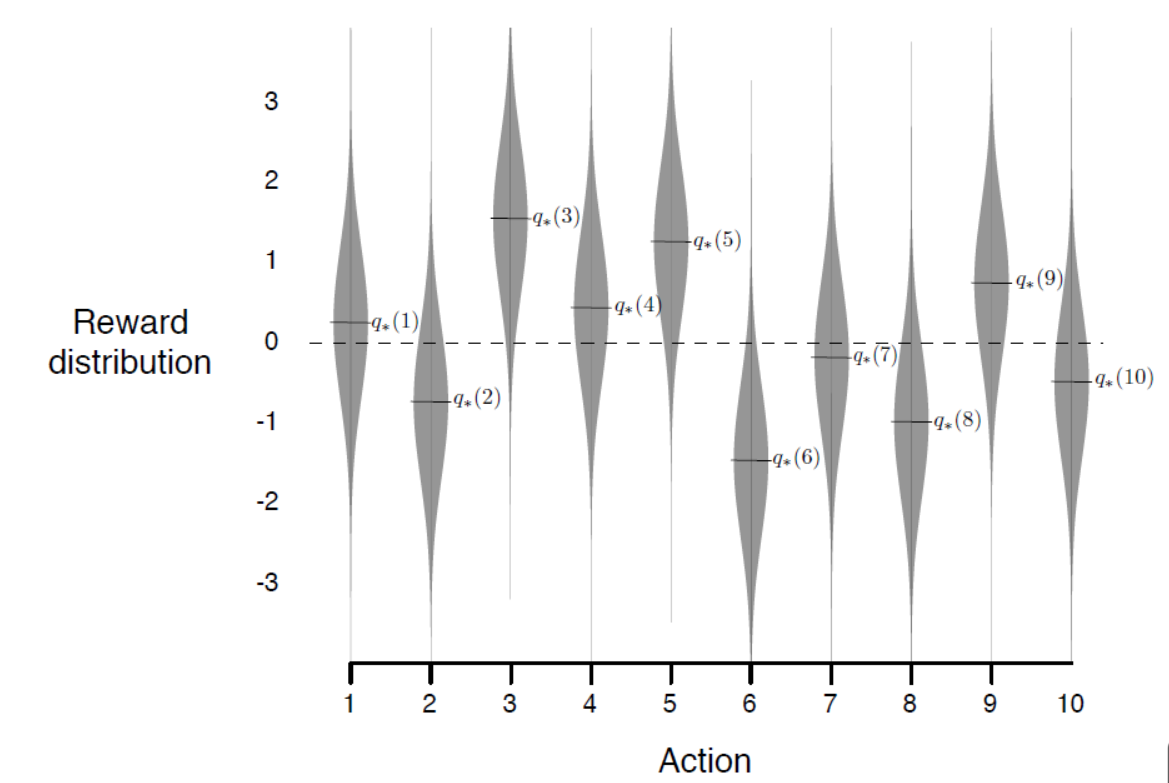
\includegraphics[width=0.6\textwidth]{f2-1}
                \caption{10臂赌博机上的一个简单案例。十个不同拉杆对应的$q_*(a)$的真实值是从一个标准正态分布中所获取的,而拉杆对应的奖励则来自于以$q_*(a)$为均值,方差为1 的正态分布,也就是图中所示的灰色分布}
                \label{f2_1}
            \end{figure}
            每一个拉杆对应的奖励抽取方法在图\ref{f2_1}中已经说明。对于任何一种学习方法,假设它使用固定的一台赌博机进行1000次的赌博,每一次赌博都有一个奖励。每进行1000次赌博,我们称为一个回合(Run)。重复2000次独立的回合,每一个回合所面临的赌博机都有所不同,那么基于这样的数据,我们就可以估计出当前学习算法的优劣程度。
            \begin{figure}
                \centering
                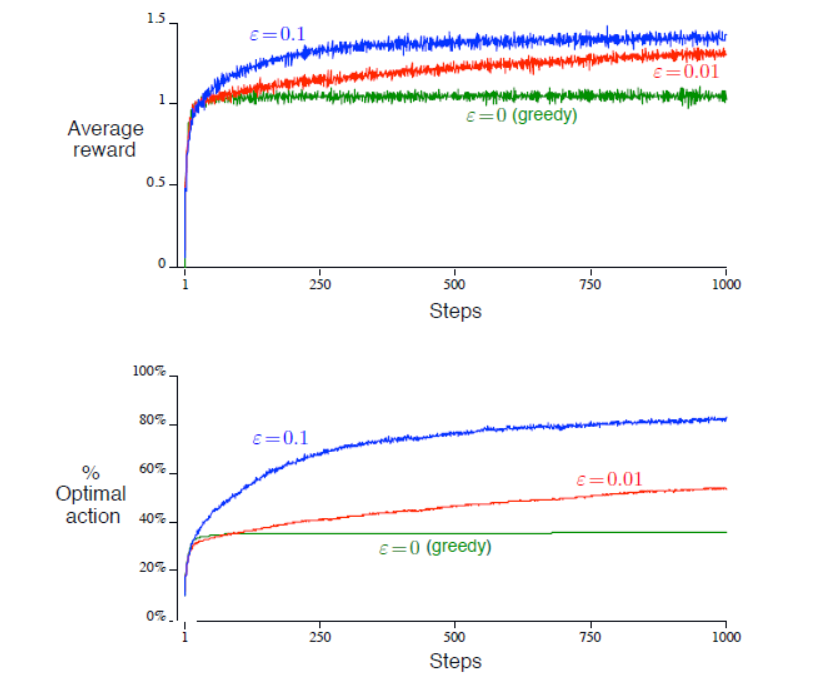
\includegraphics[width=0.6\textwidth]{f2-2}
                \caption{两千个回合中的贪心算法,$\epsilon$-贪心算法的平均性能对比。所有的方法都使用样本平均的方法来对值方程进行估计}
                \label{f2_2}
            \end{figure}
            图\ref{f2_2}在10臂赌博机上将贪心方法和两个不同水平的$\epsilon$-贪心方法($\epsilon=0.01/\epsilon=0.1$)进行了对比。这几种方法都是使用样本平均的方法来估计行动的值方程,图\ref{f2_2}中上面的子图说明了随着经验的增多,后续轮次的赌博收益逐渐增大,其中贪心方法在起始时刻的改进速度会比较快一些,但最终收敛在一个较低的水平之上,每一次赌博的回报大约稳定在1左右,而最优的方法可以达到1.5左右。在长期中,贪心方法表现很差的原因是它经常会被困在表现比较差的次优决策当中。图\ref{f2_2}中下面的子图说明贪心策略只有大致三分之一的概率可以发现最优行动决策,在其余的三分之二的情况中,它早期的关于最优行动的样本实际上是错误的,而且它也没有机会更正错误。而$\epsilon$-贪心方法在最终阶段表现较好的原因是它们持续探索并修正最优决策。$\epsilon=0.1$的情况下该方法探索得更多,也更早的找到了最优决策,不过它作出最优决策的概率不超过91\%。而在$\epsilon=0.01$时,该方法探索得速度比较慢,但最终它在上下两个指标上的表现都将优于$\epsilon=0.1$的情况。当然,如果随着决策次数的增多,逐步降低$\epsilon$是一个更好的办法。

            $\epsilon$-贪心方法要比贪心方法更好是取决于任务类型的。在奖励的波动越大的情况下,进行更多的探索行动是更有利的。相反,如果奖励的波动为零,那么仅仅一次测试就可以知道每一个行动对应的奖励,这种情况下,贪心就要比其他方法强。即便在确定情况下,只要某一些假定被弱化,进行探索行为也是有益的。比如说假设赌博机不是稳定的,每过一段时间其奖励就会变化,这种情况下就必须进行一些探索来确定最优的决策有没有发生变化。在后续章节中我们会发现,增强学习问题经常会面临这种非稳定性环境。即便说,潜在任务本身是稳定的,也是确定的,学习机也不得不面临着随之学习的进步,候选的决策空间发生了变化,对应的决策奖励也发生了变化。增强学习不得不时时刻刻在探索和压榨之间进行平衡。

        \subsection{进阶讨论}
            我们目前讨论过的值方程方法都是通过样本平均来估计行动对应的值的。接下来讨论在限定存储和决策次数的条件下如何高效计算对应的平均值。

            为了简化符号,这里只集中讨论一个行动。记$R_i$代表第$i$次执行该行动时所获取的奖励,并记$Q_n$代表在该行动出现$n-1$次之后对该行动值的估计,即:
            \begin{equation}
                Q_n \dot{=} \frac{R_1 + R_2 + \cdots + R_{n-1}}{n-1}
                \label{e_5}
            \end{equation}
            一种最简单的方法就是存储奖励的记录,然后在需要的时候执行该计算。但是这样做的话,随着决策次数的增加所消耗的存储和计算能力也会上升。

            正如你可能想到的,这样做其实是没必要的。很容易就可以将更新平均值的递增的公式更改为较小的固定计算量的计算公式。给定第$n$阶段的值$Q_n$和对应的奖励$R_n$,那么整个$n$个阶段的平均值为:
            \begin{equation}
                Q_{n+1} = Q_n + \frac{1}{n} [R_n - Q_n]
                \label{e_6}
            \end{equation}
            当$n=1$时,$Q_2=R_1$。这一实现方式只要求存储$Q_n$和$n$,每一次更新只需要简单的计算。

            形如\ref{e_6}的表达式在本书中会反复出现,通用的形式为:
            \begin{equation}
                NewEstimate \leftarrow OldEstimate + StepSize [Target - OldEstimate] .
                \label{e_7}
            \end{equation}
            其中表达式$[Target-OldEstimate]$是当前估计值的误差(error)。误差被缩放一定比例后加入到原有的估计值上,促使原有的估计值更加靠近目标值。目标值被认为是移动的正确方向,尽管它其中可能包含噪音。在上例中,目标值就是在第$n$次决策中的回报。

            有必要注意的是,递增公式\ref{e_6}中使用的步长参数($StepSize$)在每一步中都会发生变化。在处理行动$a$对应的第$n$步奖励时,该方法使用的步长参数为$\frac{1}{n}$。在本书中记步长参数为$\alpha$,或者更一般的,记为$\alpha_t(a)$。

            带有增量样本平均计算方法和$\epsilon$-贪心决策机制的完整赌博机问题解决方案的伪代码如下表所示,其中方程$bandit(a)$实现的是输入指定行动$a$,并返回对应的奖励:
            \begin{enumerate}
                \item 初始化:对于行动$a=1\ \ to\ \ k$:

                     $Q(a)\leftarrow 0$

                     $N(a) \leftarrow 0$
                \item 依次做如下循环:
                    \begin{equation}
                        A \leftarrow \left\{
                            \begin{matrix}
                                \operatorname*{argmax}\limits_{a} Q(a) & \text{概率为} 1-\epsilon \\
                                \text{随机行动} & \text{概率为}\epsilon
                            \end{matrix}
                            \right.
                    \end{equation}

                    $R \leftarrow bandit(A)$

                    $N(A) \leftarrow N(A) + 1$

                    $Q(A) \leftarrow Q(A) + \frac{1}{N(A)}[R - Q(A)]$
            \end{enumerate}
        \subsection{处理非稳定性问题}
            目前所讨论的样本平均方法只适用于稳定赌博问题,也就是说特定行动对应的奖励分布不随着时间发生变化的情况。正如之前讨论的,在增强学习问题中经常遇到的是显著的非稳定性问题。在这种情形下,近期的奖励相比于远期奖励具有更高的权重。实现这一点最普遍的方式是采用固定的步长参数。比如说公式\ref{e_6}被修正为
            \begin{equation}
                Q_{n+1} \dot{=} Q_n + \alpha [R_n -Q_n]
                \label{e2.5}
            \end{equation}
            其中的步长参数$\alpha\in (0,1]$是一个常量。这样处理之后$Q_{n+1}$就是过去样本上的加权平均:
            \begin{equation}
                Q_{n+1} = (1-\alpha)^n Q_1 + \sum_{i=1}^n \alpha (1-\alpha)^{n-i} R_i .
                \label{e2.6}
            \end{equation}
            由于$(1-\alpha)<1$,所以随着轮次的增长,早期奖励的权重逐步缩减到0,而且这一缩减速度是指数倍的,故这一方法也被称为指数衰减加权平均。

            有时,在每一个轮次动态调整步长参数也是可行的。记行动$a$第$n$次出现后对应的步长系数为$\alpha_n(a)$。已知当$\alpha_n(a)=\frac{1}{n}$时对应着样本平均方法,同时根据大数定律可以保证估计值收敛到真实值,但是并不是说从函数空间$\{\alpha_n(a)\}$中任意选择一个方程就能够保证收敛的。在随机逼近理论中有一个很经典的结论,观测序列和向潜在和值收敛的前提条件是:
            \begin{equation}
                \sum_{n=1}^{\infty} \alpha_n(a) = \infty \qquad and \qquad \sum_{n=1}^{\infty} \alpha_n^2(a) < \infty
                \label{e2.7}
            \end{equation}
            前一个假设保证了权重系数足够大,以至于后期的值能够抵消前期任意初始值的影响,而后一个假设保证逼近稳态值之后可以收敛。

            在样本平均方法中,收敛条件的两个假设都是满足的;而在固定步长的情况下,收敛条件的第二个假设是不能满足的,也就是说结果用于都不会收敛,而会随着最近的值而波动。不过之前已经讨论过,这一点正是非稳定环境下所必须的,而这种非稳定环境也是增强学习经常碰到的。另外,即便说权重序列满足公式\ref{e2.7} 所要求的,那么最终的收敛可能也是很慢的,需要非常精细的调节才有可能达成合理的收敛速度。所以说尽管符合收敛条件的权重序列在理论研究中使用的很多,但是在实际运用中很少使用。

        \subsection{最优初始值}
            目前讨论的方法都在一定程度上依赖于初始值$Q_1(a)$的设定。用统计学的术语来说,就是这些方法都是有偏估计。在样本平均方法中,只要所有的行动都被选中了一次,这种偏置就被消除了,而在固定步长时,尽管偏置会根据公式\ref{e2.6}以指数速度下降,但是初始值的影响永远都无法消除。实际上,这种偏置在很多情况下不是一种问题,反而很有用。这一影响不好的一面是初始的估计值需要建模人员去精心挑选,除非全设置成零。但好的一面是这是一种非常便捷的将先验信息放入到模型当中的方法。

            初始值的设置也可以用来鼓励探索行为。假设在10臂赌博机的值方程初始值设定上设定的不是0,而是5的话,而潜在的真实回报均值$q_*(a)$是服从标准正态分布的,所以初始值5大概率是好于真实均值的,那么学习机在尝试了一个行动之后,得到的回报低于5,那它就会去尝试那些未被尝试的行动,这样的话,即便是使用贪心决策方法,所有的行动也都会被尝试几次。

            图\ref{f2_3}展示了在10赌博机上对比两种方法的结果,一种是初始值为5的完全贪心决策方法(称为正向初始值方法),而另一种是初始值为0的$\epsilon$-贪心决策方法。最开始,第一种方法表现比较差,因为它进行了很多的探索,但是在长期中它表现更好,因为长期之后它基本上不再进行探索行为。我们将这种鼓励探索的技巧称为正向初始值方法。一般认为,该方法在稳定环境下具有很高的效率,但是本质上它并不是一种鼓励探索行为的方法。比如说,它就不适用于非稳定问题,因为它对于探索行为的偏好只是临时性的。
            \begin{figure}
                \centering
                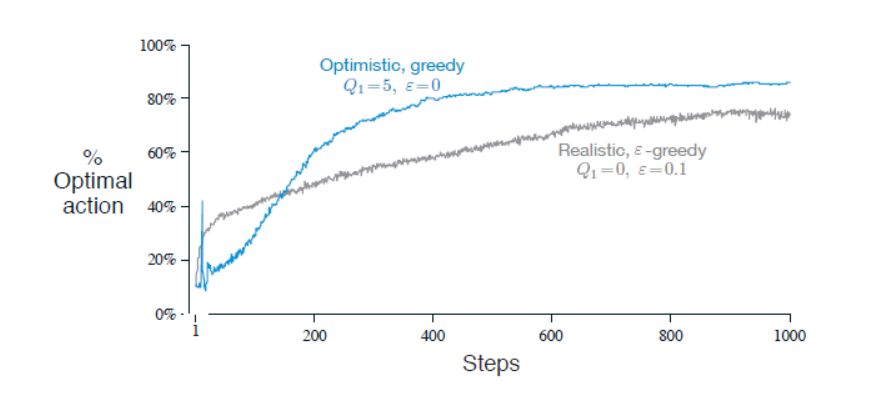
\includegraphics[width=0.6\textwidth]{f2-3}
                \caption{在10臂赌博机上正向初始值贪心方法和$\epsilon$-贪心方法的效果对比,这两种方法都采用固定步长,$\alpha=0.1$}
                \label{f2_3}
            \end{figure}
            如果环境发生了变化,这就需要重新进行探索,但该方法并不会诱使探索行为的出现。更一般来说,任何在初始值上做功课的方法都无法应对非稳定环境问题。由于起始状态只会出现一次,所以没有必要太关注。这一点同样适用于样本平均方法,该方法也同样始终保留初始观测的影响。尽管如此,这些方法是很简单的,它们当中的任何一个或者多个的组合在实际应用中是足够的。在本书的后续部分也会多次用到这些简单的触发探索的技巧。

        \subsection{基于置信上界的行动选择方法}
            探索行为总是必要的,因为在过程中始终对值方程的估计值不确定,所谓的占优决策也只是基于已有的信息,可能存在潜在的更优的决策。$\epsilon$-贪心方法将其他的非占优决策等同视之,没有参考当前行动的值或者不确定性等信息。最好的想法是充分利用每一个非占优决策离最优决策值的距离,以及相应的非确定性来选择探索哪一个非占优决策。有一个很有效的方法是基于下式:
            \begin{equation}
                A_t \dot{=} \operatorname*{argmax}\limits_{a} [Q_t(a) + c\sqrt{\frac{\ln t}{N_t(a)}}]
                \label{e2.10}
            \end{equation}
            其中$\ln t$表示轮次$t$的自然对数,$N_t(a)$代表行动$a$在$t$个轮次中出现的次数。而参数$c$则控制了探索行为的强度,如果$N_t(a)=0$,那么就认为行动$a$具有最大的值。

            利用上述公式来产生决策的方法被称为置信上界(Upper Confidence Bound,UCB)确定决策方法,其中的带根号的部分反映了当前对于行动$a$的值的估计的不确定性。公式\ref{e2.10}可以视为对于行动$a$潜在的值的可能上界,其中参数$c$衡量了不确定性在这其中的影响力。每一次$a$被选中之后,其对应的不确定性就会下降:$N_t(a)$增大之后,,由于它出现在分母上,所以不确定那一项会减小。反之,当行动$a$之外的其他行动被选中,那么行动$a$对应的不确定性会增大。其中使用的自然对数使得轮次$t$的增长在不确定性中的作用逐步降低,但是并无上限。根据上述公式可以,所有的行动都会被选中,但是那些值较低的,或者已经被选中很多次的行动在后续轮次中被选中的概率会大大下降。

            UCB方法在10臂赌博机上的试验结果在图\ref{f2_4}中展示。从图中可以看出,UCB方法整体上是优于$\epsilon$-贪心方法的,但是很难从多臂赌博机的问题推广到其他更一般的增强学习问题上。第一个困难是处理非稳定环境问题,另一个困难是处理状态空间巨大的情况。在这些复杂情况下,UCB的方法是实际中是效果不好的。
            \begin{figure}
                \centering
                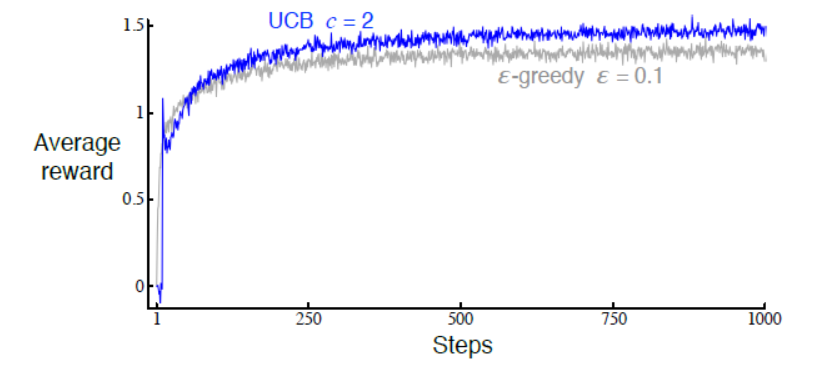
\includegraphics[width=0.6\textwidth]{f2-4}
                \caption{UCB方法在10臂赌博机进行试验的平均结果。可以看出,除了在最开始的$k$个阶段,它需要尝试不同的行动方案,所以性能不太好,在后期的性能要优于$\epsilon$-贪心方法}
                \label{f2_4}
            \end{figure}

        \subsection{梯度赌博方法}
            本章我们已经学习了多种估计值方程的方法,以及基于这些方法来进行决策。这些方法是很好的方法,但是并不是唯一的方法。本节将讨论如何给每一个行动赋予一个优先值,记为$H_t(a)$。这种优先值越大,采取这种行动的频率就越高。但是这种优先值不能用奖励来解释,只有一个行动和另一个行动的优先值的相对大小才有意义,比如说,把所有行动的优先值都增加1000,那么选择各个行动的概率不会发生变化。基于优先值来计算行动概率的方法是使用Soft-Max函数:
            \begin{equation}
                Pr\{A_t = a\} \dot{=} \frac{e^{H_t(a)}}{\sum_{b=1}^k e^{H_t(b)}} = \pi_t(a).
                \label{e2.11}
            \end{equation}
            这里我们引入了一个新的重要记号$\pi_t(a)$,代表该轮次采取行动$a$的概率。最开始的时候,所有的行动都有相同的优先值,比如对于任意的行动$a$,都有$H_1(a)$,故所有的行动都有相同的被选中的概率。

            基于随机梯度下降方法的思想,实现这一想法有一个自然的算法,在每一步选中了行动$A_t$之后会受到奖励$R_t$,那么行动的优先值就使用如下方式进行更新:
            \begin{equation}
                \begin{split}
                    &H_{t+1}(A_t) \dot{=} H_t(A_t) + \alpha(R_t-\bar{R}_t)(1-\pi_t(A_t)) \\
                    &H_{t+1}(a) \dot{=} H_t(a) - \alpha (R_t - \bar{R}_t)\pi_t(a) \qquad \qquad for\ \ all \ \  a\ne A_t
                \end{split}
            \end{equation}
            其中$\alpha > 0$是步长参数,$\bar{R}_t\in \mathbb{R}$是截止到(并包括)轮次$t$为止每一个轮次的平均奖励,它是每一个行动所获奖励进行对比的基准线。如果行动$A_t$对应的奖励$R_t$大于基准线,那么在后续轮次中采取该行动的概率就会上升,反之,就会下降。没有被选中的行动则会反方向变动。

            图\ref{f2_5}展示了梯度赌博算法在10臂赌博机上的效果,不过在这次试验中,奖励均值的来源分布变为均值为4,方差为1的正态分布。这种所有奖励的平移对于梯度赌博算法是没有影响的,因为奖励的基准线也会上移到同一水平之上。但如果忽视了基准线,也就是说$\bar{R}_t=0$,那么该方法的表现就会大大下降,正如图中所示。
            \begin{figure}
                \centering
                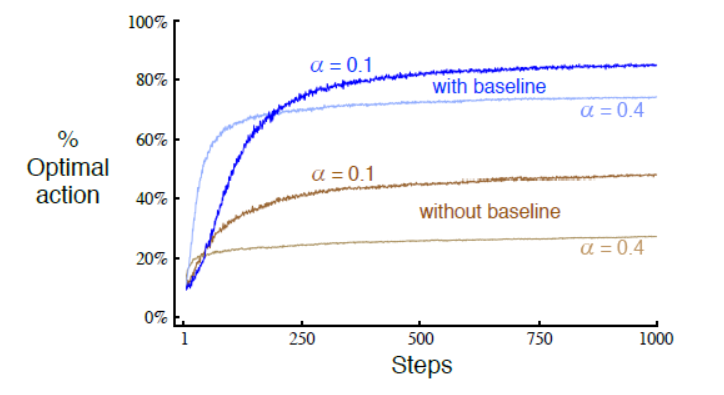
\includegraphics[width=0.6\textwidth]{f2-5}
                \caption{梯度赌博算法在考虑基准线和不考虑基准线两种情况下的平均性能}
                \label{f2_5}
            \end{figure}

        \subsection{耦合搜索(时序依赖的赌博机)}
            到目前为止我们所考虑的是只是无时序依赖的问题,或者说,那些不需要考虑将不同状态下不同行动结合在一起考虑的问题。在这一类任务中,学习机企图在环境稳定的状态下确定最优的单个行动,或者说在环境不稳定的情况下,能够追踪最好的单个行动。但是,在增强学习任务中很多的情况是状态空间很大,而目标是学习一种决策机制:可以从状态映射到一个最佳行动的函数。这里我们简单讨论一下如何从非耦合任务拓展到耦合任务中。

            举一个例子,假设有几个不同的$k$-臂赌博机,每一次决策时都随机选择一个赌博机。因此,每一步中赌博机都在发生随机变化。这看起来就好像是你面对着一个单独的,不稳定的多臂赌博机,这一台赌博机每一轮次的行动的值都随机变化。你可以尝试本章讨论的各种方法去处理这种非稳定的局面,但是除非行动的值的变化是很缓慢的,那么这些方法效果都不好。但是现在假设当随机选定一台赌博机之后,你可以获得一些特别的线索去判别它是哪一台,但是无法获知它之上行动的实际值。比如说,赌博机在发生变化的时候,界面的颜色也会随之变化。那么你就需要额外学习一个策略,根据所看到的颜色不同,来为相同的状态指定不同的决策方案,比如如果界面是红色的,就拉动拉杆1,如果是绿色的,就拉动拉杆2。只要能采取正确的策略,就可以获取到比忽略这些区分信息更好的决策效果。

            这是耦合搜索任务的一个例子,之所以这么说是因为它同时涉及到根据试错学习来确定最优的行动和将这些行动与环境相结合来选择最优行动。耦合搜索任务在论文中通常被称为时序依赖赌博机问题。耦合搜索任务实际上是介于多臂赌博机和标准增强学习问题之间的一个问题,它需要学习到一个完成的策略,这与标准的增强学习比较类似,但是由于每一轮次的行动只影响当前的奖励,这又不同于标准增强学习。如果所选中的行动不仅影响当前的奖励,也会影响未来的状态,那么这就是一个标准的增强学习问题了。我们会在下一章提出这一问题并考虑它的影响。

        \subsection{总结}
            本章中我们提出了几种可以平衡探索和压榨的方法。其中$\epsilon-$贪心方法随机地选择一定比例的轮次来进行探索,而UCB方法使用一种确定的方法来实现探索,并且隐式地促使学习机探索出现次数较少的行动。梯度赌博算法并不是估计行动的值,而是估计行动的优先值,并基于优先值使用SoftMax分布来随机选择行动。简单地通过将行动的初始“值”设置为正数的方法可以促使即便是完全贪心方法也会进行充分的探索。

            很自然的,我们想要知道哪一种方法是最好的。尽管这一问题很难回答,但是可以在10臂赌博机进行足够多次的试验之后对比就可以知道哪一个方法更好。一个难点是,每一种方法都涉及到几个参数,为了获得有意义的比较结果,就必须寻找每一种方法的最优参数,然后基于最优参数来对比各个模型的优劣。图\ref{f2_6}中对比了几种不同的方法在不同参数设置下的性能,从图中可以看出,性能曲线都是倒U型的,即最优性能出现在核心参数既不太大也不太小的情形下。
            \begin{figure}
                \centering
                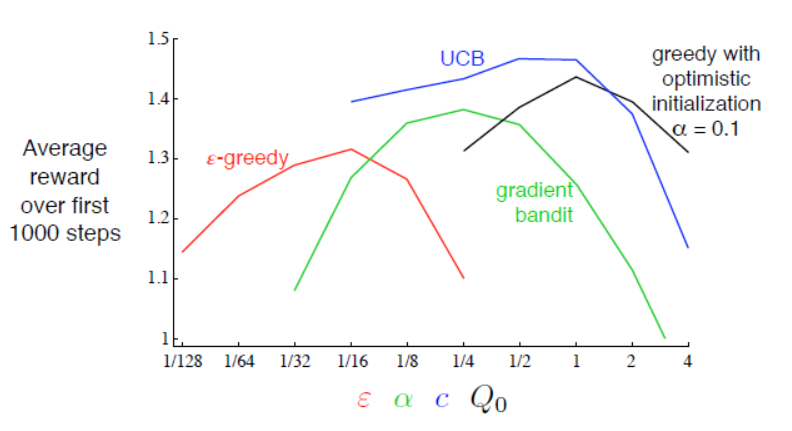
\includegraphics[width=0.6\textwidth]{f2-6}
                \caption{本章所讨论的各种赌博机算法的参数研究,每一个点上的值都是特定的算法在特定的参数设置下1000个轮次奖励的平均}
                \label{f2_6}
            \end{figure}
            在评估一个模型时,我们不应该只考虑模型在最优参数时的性能,也应该考虑模型性能对应参数的敏感性。从图上对比可以看出,这几个模型对于参数的敏感性大致相同。因此从全局来看,就这个问题而言,UCB方法是性能最好的。

            经过本章介绍的方法都比较简单,但是这些方法都是非常好的。有一些更复杂的方法,但他们的复杂性和假设使得他们在标准的增强学习问题中不具备实用性。在第五章讨论标准的增强学习问题时我们会用到这些简单的方法。

            在多臂赌博机上有一种很好的可以平衡探索和压榨的方法可以计算出一种特殊的行动值,叫做Gittins Index。在某些特殊情况下,这种计算很简单,也可以直接指向最优解,但它要求能够知道值的完整的先验分布,当然这实际上通常是不可行的。另外,无论是这种方法的理论还是计算上的简便性都无法推广到标准增强学习问题上。

            Gittins-Index方法是贝叶斯方法的一个案例,贝叶斯方法通常假设知道行动值的初始分布,然后在每一个轮次中更新该分布。一般来说,这种更新计算是很复杂的,但对于某些特殊的初始分布(称为共轭分布)可以简化计算。一种可能是根据后验分布来决定每一个轮次所选择的最佳行动。这种方法一般称为后验分布采样,基本上和最好的无分布方法的效果类似。

            在贝叶斯设定下,甚至可以计算出最优的探索和压榨的比例。基于奖励的分布,学习机可以计算出每一个行动对应不同奖励的概率,以及出现不同奖励之后进一步的后验分布情况。所涉及的这个分布变成了问题的信息状态。给定一个界限,比如1000个轮次,学习机可以考虑所有可能的行动,以及对应的奖励,以及进一步的可能行动,以及进一步的奖励,一直将1000个轮次迭代完毕。但是这种概率树的规模增长是极为迅速的,不太可能做如此大规模的计算,但是,这种方法可以在一定程度上被高效的近似。这种方法可以迅速地将赌博机问题转变为一个标准的增强学习问题。最后,我们可以使用第二部分所讨论的近似增强学习方法来逼近最优解,不过这是研究的前沿,超出了本书作为一本入门读物的要求。

    \section{有限马尔科夫决策过程}
        本章会介绍有限马尔科夫决策过程(finite MDPs)的标准形式。这一问题涉及到可评估的反馈,和耦合问题--也就是在不同的状态下要选择不同的行动。MDPs是一种典型的序列决策模型,其行动不仅影响当前的奖励,也会影响后续的状态,进而影响后续的奖励。因此MDPs问题涉及到延迟的奖励和需要在即刻奖励和远期奖励之间进行平衡。尽管在赌博问题中估计了值方程$q_*(a)$,但在MDPs需要估计基于状态$s$和行动$a$的值方程$q_*(s,a)$,或者我们估计的是基于最优行动的值方程$v_*(s)$。这些依赖于状态的量对于准确的确定长期行动选择具有很重要的作用。

        MDPs方法是增强学习问题最理想的数学形式,在该形式下,可以计算出每一个状态精确的理论值。本章引入该问题数学结构的关键元素,比如回馈,值方程和Bellman 方程。本章会将很多的应用转换为标准的有限MDPs形式。在所有的人工智能领域中,模型的适用性和数学上的简易性两者不可兼得。本章会介绍这种矛盾以及对应的折中方法和挑战。MDPs方法之外的一些增强学习手段会在第17章讨论。

        \subsection{学习机-环境交互接口}
            MDPs方法是一种直观的从交互中进行学习以达成目标的分析框架。学习机器或者说决策者这里记为Agent,与Agent相交互的所有一切外部事物所构成的整体称之为Environment。随着交互的进行,Agent确定Action,Environment对Action进行响应,然后转换为新的Situation提供给Agent。Environment同时会反馈一个Reward,这个Reward是一个特殊的数值,Agent尝试随着轮次的进行通过选择不同的Action来获取最大的Reward总和。
            \begin{figure}
                \centering
                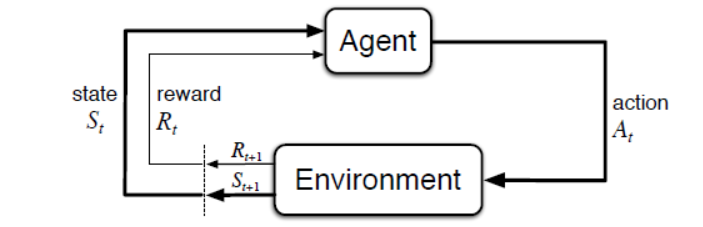
\includegraphics[width=0.6\textwidth]{f3-1}
                \caption{在马尔科夫决策过程中Agent-Environment之间的交互}
                \label{f3_1}
            \end{figure}

            更特殊的是,Agent和Environment之间的交互是建立在一组离散的时间序列$t=0,1,2,\cdots$之上,在每一离散时间步$t$之上Agent可以获得到Environment的状态值($S_t \in \mathbb{S}$),基于该Situation,Agent从一组可选Action中选择一个,即$A_t \in \mathbb{A}(S_t)$。在Action结束之后,Agent会获得到一个数值型的Reward,即$R_{t+1} \in \mathbb{R}$,然后环境进入一个新的状态$S_{t+1}$。马尔科夫决策过程和Agent结合在一起就构成了如下的序列:
            \begin{equation}
                S_0,A_0,R_1,S_1,A_1,R_2,S_2,A_2,\cdots
                \label{e3.1}
            \end{equation}
            在有限马尔科夫决策过程,State,Action以及Reward的集合都是有限的,在这种情况下,随机变量$R_t$和$S_t$在给定特定的State和Action之后服从严格的离散概率分布。也就是说,特定的下一轮次状态$s'\in \mathbb{S}$和奖励$r\in \mathbb{R}$,在给定当前的State和Action之后,其出现的概率为:
            \begin{equation}
                P(s',r|s,a) \dot{=} Pr{S_t=s',R_t=r | S_{t-1}=s,A_{t-1}=a}
                \label{e3.2}
            \end{equation}
            其中$s',s\in \mathbb{S},r\in \mathbb{R},a\in \mathbb{A}$。概率方程$P$定义了MDP过程的动态性,这一动态方程是一个常规的带有四个参数的判别式方程。当然,这里的概率方程符合归一性,即对于任何的$s$与$a$,有:
            \begin{equation}
                \sum_{s'\in \mathbb{S}}\sum_{r\in \mathbb{R}} P(s',r|s,a) = 1,\ for all s\in \mathbb{S},a\in \mathbb{A}(s)
                \label{e3.3}
            \end{equation}

            在马尔科夫决策过程中,由$p$所定义的概率完全刻画了Environment的动态性,也就是说,$S_t$和$R_t$可能值的概率仅仅依赖于即刻的State,$S_{t-1}$和Action,$A_{t-1}$,而跟之前的State和Action都无关。最简单的理解就是该轮次的概率方程$P$只依赖于State,而不依赖于行动序列。那也就是说,State就必须包含了能够影响未来的过去的Agent-Environment之间交互的全部信息,如果这一点可以达成的话,那么就称这种State具有马尔科夫属性。尽管从第二部分会开始研究不依赖于马尔科夫性的近似方法,在第17章会讲解如何从一个非马尔科夫过程的基础上去构建马尔科夫过程,但本书还是认为马尔科夫性质这一要求贯穿全书。

            基于四参数的动态方程$P$可以计算出关于Environment的全部信息,比如状态转移矩阵(state-transition probabilities):
            \begin{equation}
                P(s'|s,a) \dot{=} Pr\{S_t=s'|S_{t-1}=s,A_{t-1}=a\} = \sum_{r\in R} P(s',r|s,a)
                \label{e3.4}
            \end{equation}
            同样可以计算出State-Action对对应的期望收益:
            \begin{equation}
                r(s,a) \dot{=} \mathbb{E} [R_t|S_{t-1}=s,A_{t-1}=a] = \sum_{r\in \mathbb{R}} r \sum_{s'\in \mathbb{S}} P(s',r|s,a)
                \label{e3.5}
            \end{equation}
            或者是计算出(State,action,next-state)三个特征所对应的期望收益:
            \begin{equation}
                r(s,a,s') \dot{=} \mathbb{E} [R_t|S_{t-1}=s,A_{t-1}=a,S_t=s'] = \sum_{r\in \mathbb{R}} r \frac{P(s',r|s,a)}{P(s'|s,a)}
                \label{e3.6}
            \end{equation}
            本书中我们经常会用到公式\ref{e3.2},不过其他几个公式有时很方便。

            MDPs框架抽象,自由度大,可以以不同的方式应用于很多不同的问题上。比如时间间隔不需要是固定的;它可以在任何后续阶段上进行决策和行动。行动可以在较低的层级上进行控制,比如输入到机械手臂发动机上的电压,或者在很高的层级上,比如说是否吃午饭或者是否上研究生等等。相似的,State可以采用各种各样的形式,低层级上可以是传感器的读数,或者在一个很高的或者抽象的层级上,比如对一个房间内的物体进行符号化描述。构成State的一些元素可能是基于传感器之前存储的值,甚至完全是精神上的或者是主观上的,比如Agent可以处以不确定对象具体位置或者是某一些传感器读数故障的State下。相似的,有一些Action 可能完全是主观性的,或者是估计的,比如有一些Action就是控制Agent去思考,或者决定它注意力集中的位置。一般来说,Action可以是任何一种待学习的决策方法,State可以是任何一种会影响Action选择的指标。

            具体而言,Agent和Environment之间的界限并不像机器或者动物的实体一样分割清晰。一般来说,这个界限更靠近Agent一些。比如机器人的发动机,机械连接装置,以及传感器等通常被认为是Environment的一部分,而不是Agent的一部分。相似地,如果将MDPs方法应用于人或者动物,那么肌肉,骨骼,或者感知器官都属于Environment的一部分。Reward也是一样,如果是生物体,Reward通常是由生物体内部所衡量的,但是在智能系统中,Reward是在智能体外部所计算的。

            一般这样认为,Agent不能任意控制的元素都认为是外部元素,也就是Environment的一部分。比如,Agent多多少少是知道一些如何基于Action和State来计算Reward的方法,但是呢,总是将Reward的计算认定是Agent的外部因素,这是因为Reward本身就规定了Agent所要优化的任务,所以Agent是不能任意的设置Reward 的值的。实际上,在有一些情况下,Agent完全了解其相应的Environment,但是完成增强学习任务还是有较大的困难,就比如说你知道魔方的一切规则,但是你还是解决不了这个问题。总之,Agent和Environment之间划分界限的标准不是Agent能够感知到的范围,而是Agent所能绝对控制的范围。

            Agent和Environment的边界处于不同的目的可以划分在不同的位置。在一个复杂的机器系统中,可以有很多不同层级的Agent同时工作,每一个都有自己的边界。比如说,有一个Agent在较高的层级作出决策,这一决策构成了低层级Agent的环境,在这样的环境里,低层级Agent来实现高层级Agent的决策。在实际工作中,当选定了状态空间,行动空间和回报机制之后,就确定了Agent所要完成的具体任务,Agent的界限就确定了。

            MDPs框架是对通过交互进行目标导向学习的问题的高度抽象。该模型认为,无论传感器,存储,或者控制单元的具体形式,也无论目标是如何达成的,任何目标导向的学习问题都可以被简化为三个信号在Agent和Environment之间进行传递,一个信号代表Agent的Action,一个信号代表作出Action的基础,也就是Environment的State,另一个信号就是Agent的目标,也就是Reward。这一框架并不能完全表达决策学习问题的各个方面,但是已被实践证明这一方法是有用且广泛适用的。

            当然,由于任务的不同,State和Action的具体表现形式有很大的不同,其表达方式的优劣会很大程度上影响模型的效果。同其他学习方法一样,增强学习如何对各个State,Action进行表示是一件极富有灵感的任务,没有一定的规律可循。本书会提到一些建议和例子来说明如何较好的表示State和Action,但是核心内容还是基于表示方法已经确定的基础上如何进行学习的问题。

        \subsection{目标和奖励}
            在增强学习中,Agent的目标或者目的被形式化的表述为一组的特殊信号,称为Reward,它被从Environment传递给Agent。每一个轮次中,Reward是一个简单的数字$R_t\in \mathbb{R}$。不严谨地说,Agent的目标就是最大化其所获得Reward的总和。也就是说,Agent的目标不是最大化即刻Reward,而是最大化在长周期中的Reward总和。将这种非正式的相反可以表述为如下的Reward假设:

                \begin{quote}
                  所谓的目的或者目标也就是最大化所收到的标量信号(Reward)的累积总和的数学期望。
                \end{quote}

            使用Reward信号来刻画目标是增强学习的核心特点之一。

            起初来看,将目标分解为Reward信号局限性很大,不过在实际应用中,这种方法被证明具有很大的适用性和自由度。举个例子来说,为了指导机器人学会走路,研究人员在每一个轮次根据机器人向前移动的步长成比例的给予Reward信号;为了教会机器人如何从迷宫中逃离,那么Reward信号被设置为在逃离迷宫之前每过一个轮次就给予一个-1,这样的Reward信号鼓励Agent在尽可能少的轮次中逃离迷宫;为了促使机器人收集更多的空汽水罐,那么在大部分轮次中机器人所获得的信号都是0,而当它在收集到一个空罐子的时候,Reward信号就变为1,或者在机器人撞到某东西,或者被人指责时,就会接收到一个负值的Reward;为了教会一个机器人下棋,那么就在它获胜的情况下给予Reward$+1$,而在它失败的时候给予Reward$-1$,而平局或者还未结束的情况下Reward是$0$。

            从以上的例子可以发现,Agent总是尝试最大化它的Reward。如果我们想促使Agent为我们实现某项功能,我们就必须为Agent提供一种Reward信号,Agent最大化这一Reward信号,就可以达成那一项功能。所以设置的奖励信号就必须和目标之间具有强烈的关联性。实际上,Reward信号并不是说给Agent提供先验信息来告诉它做哪一些事情可以达成我们想要的目标。比如说,下棋Agent所获得Reward信号仅仅发生在它实际取得胜利的情况下,而不是在它达成某一个子目标的时候,比如吃掉对面的一个棋子或者控制了棋盘的中心位置。如果达成这些子目标同样可以获得Reward,那么Agent可能就不会去完成真正的目标。比如说,Agent可以会优先去吃掉对方的棋子,尽管代价有可能是输掉比赛。Reward信号一定是你所要想Agent达成的目标,而不是Agent达成目标的方法。

        \subsection{回报和回合}
            截止当前,本章已经非正式地讨论了学习的目标。之前已经陈述过,Agent的目标是最大化在长期中所接收到的累积Reward总和。那么如何正式地定义这一点呢?在轮次$t$之后所获得的Reward序列记为$R_{t+1},R_{t+2},R_{t+3},\cdots$,那么这一个序列中的哪一部分是期望最大化的呢?一般来说,希望能最大化期望收益,记为$G_t$,是定义在Reward序列上的某一特定函数。最简单的情形就是求和形式:
            \begin{equation}
                G_t \dot{=} R_{t+1} + R_{t+2} + \cdots + R_{T}
                \label{e3.7}
            \end{equation}
            其中$T$是最后一个轮次。这种方式在最终轮次有一个自然明确的记号是比较适用,也就是说,当Agent和Environment之间的交互可以自然的切分为序列,这里把这些序列称为回合(Episodes),比如下棋,走迷宫,或者说其他类型的重复交互。回合会以一个特殊的状态(最终状态)结束,而后就又回到了标准的开始状态,或者是回到服从某一分布的随机起始状态。即使说回合可能以不同的状态结束,比如在下棋中有赢有输,但是下一回合的起始状态是独立于上一回合的结束状态的。所以说可以认为一个回合总是在同一个状态组中结束,不同的组内具体状态对应着不同的Reward。带有回合的任务被称为回合制任务,在这一类任务中,需要对非终止状态和终止状态进行区分,非终止状态记为$\mathcal{S}$,而终止状态记为$\mathcal{S}^+$。回合结束的轮次$T$通常是一个随机变量,在每一个回合的值都有所不同。

            另一方面,Agent-Environment之间交互的很多案例不能自然地切分为可识别的回合,而是持续的无限制的进行下去。比如说运行当中的流程控制任务,或者说是长生命周期的机器人,这一类任务称为持续性任务。在这一类任务下公式\ref{e3.7}所定义的回报就有问题了,因为这个Reward序列会无限长,进而就导致其加总之和为无限大,也就无法求最大值了。因此在本书中会采用回报的另一种定义方法,这种方法在概念上比较复杂,但是在数学上比较简单。

            另外一个重要的概念是贴现的概念。在该方法中,Agent尝试选择那些可以最大化已贴现奖励总和的Action。具体来说,所选取的行动$A_t$可以最大化以下的期望贴现回报:
            \begin{equation}
                G_t \dot{=} R_{t+1} + \gamma R_{t+2} + \gamma^2 R_{t+2} + \cdots = \sum_{k=0}^{\infty} \gamma^k R_{t+k+1}
                \label{e3.8}
            \end{equation}
            其中$\gamma$是一个参数,$0\le \gamma \le 1$,被称为折现率。

            折现率决定了未来奖励的当前值。如果$\gamma<1$,且奖励序列$\{R_k\}$是有上界的,那么公式\ref{e3.8}的和就是有限的。如果折现率是0,那么Agent就是短视的,只关心眼下的利益。当然如果每一轮次的行动只决定下一轮次的奖励,而不影响进一步的奖励,那么Agent的这种短视行为就是合理的。但一般而言,过于短视的Agent往往不能得到很大的长期回报。当折现率接近1时,Agent就更看重未来的奖励,也就是特别的高瞻远瞩了。

            前后两个轮次的回报是有递归关系的:
            \begin{equation}
                G_t \dot{=} R_{t+1} + \gamma G_{t+1}
                \label{e3.9}
            \end{equation}
            上式中要求$t <T$,即便$t+1$是最后一个轮次,那么只要定义$G_T=0$,上式就一直成立。这一定义方式可以简化从奖励序列中计算回报的过程。

        \subsection{回合制和持续制任务的统一符号}
            上一节提出了两种增强学习范式,一种是Agent和Environment的交互可以自然地被切分为多个相对独立的回合,而另一种整个交互过程会一直持续下去,无穷无尽。前一种形式的问题在数学上比较简单,因为一个Action只影响有限个后续奖励。本书中有些案例是第一类问题,也有一些案例是第二类问题,也有两者相结合的形式。因此我们希望能在统一的符号体系对这两个类型的问题进行表述。

            为了准确刻画回合制任务需要增加一些新的符号。在回合制任务中需要首先考虑一系列的回合,每一个回合中也有有限个行动轮次,而不是简单地由一组很长的行动轮次所构成。也就是说不能简单的将轮次$t$的状态记为$S_t$,而应该记为$S_{t,i}$,指的是第$i$回合中的第$t$个轮次的状态,同样,定义了$A_{t,i},R_{t,i},\pi_{t,i},T_i$。不过事实证明在讨论回合制任务时基本上是不需要对不同的回合进行区分的,总是考虑一个回合就可以了。故在实际工作中我们经常会忽略到符号下标中标识回合号的符号,也就是说,$S_t$指的是$S_{t,i}$。

            同样需要遵循同一个惯例来简化符号,同时涵盖回合制任务和持续型任务。在公式\ref{e3.7}和公式\ref{e3.8}中分别定义了回报是有限个以及无限个奖励的加总和。这两类问题可以通过假设回合制任务在最后一个阶段对进入到一个特殊的状态,自吸收状态(Absorbing State),在这个状态下Agent也只能转移到这一状态,并且对应的奖励是0。也就是如图\ref{f3_1_1}所示。
            \begin{figure}[h]
                \centering
                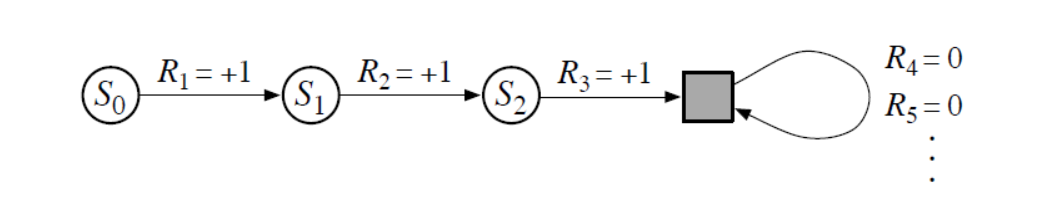
\includegraphics[width=0.6\textwidth]{f3-1-1}
                \caption{回合制任务在最后进入了自吸收状态}
                \label{f3_1_1}
            \end{figure}
            在上图中最后的实心方块代表特殊的自吸收状态。从状态$S_0$开始,我们可以获得奖励序列$+1,+1,+1,0,0,0,\cdots$,将这些值相加,结果和前$T$个轮次的求和结果相同。这一点在引入折现率之后也是成立的。有了这个定义之后,可以将回合制任务和持续型任务的回报统一定义为如下的形式(忽略回合的下角标):
            \begin{equation}
                G_t \dot{=} \sum{k = t+1}^T \gamma^{k-t-1} R_k
                \label{e3.11}
            \end{equation}
            这其中包括$T=\infty$和$\gamma=1$的可能性。

        \subsection{策略和值方程}
            基本上所有的增强学习问题都涉及到对值方程进行估计--所谓的值方程,就是估计一个状态(或者状态-行动对)对于Agent而言有多好的函数,这里所谓的多好,就是未来的回报总和有多大。当然Agent在未来所获得到的奖励依赖于其在未来的行动,相应地,值方程的定义是基于一种特定的行动决策机制,这种机制也叫做策略。

            正式而言,所谓的策略就是从状态映射到各个行动被选中的概率的函数。如果Agent在时点$t$遵循策略$\pi$的话,那么符号$\pi(a|s)$代表在状态$S_t=s$时采取行动$A_t=a$的概率。跟$p$一样,$\pi$就是一个普通函数,函数定义$\pi(a|s)$中的$|$仅仅是指该函数为每一个状态$s\in \mathcal{S}$定义了其行动$a\in \mathcal{A}(s)$的概率分布。增强学习方法会指出Agent的策略如何随着经验的变化而变化。

            在策略$\pi$下的某一状态$s$的值方程记为$v_{\pi}(s)$,代表的是从状态$s$开始,依据策略$\pi$来选择行动,那么期望回报是多少。对于MDPs,可以将$v_{\pi}$正式定义为:
            \begin{equation}
                v_{\pi}(s) \dot{=} \mathbb{E}_{\pi}[G_t|S_t=s] = \mathbb{E}_{\pi}[\sum_{k=0}^{\infty}\gamma^k R_{t+k+1}|S_t = s],\ \ for \ all \ s \in \mathcal{S}.
                \label{e3.12}
            \end{equation}
            当然,最终状态的值方程一定是0。我们将函数$v_{\pi}$称为\textbf{在策略$\pi$下的状态值方程}。

            同样,在策略$\pi$下定义的行动-状态对$(a-s)$值方程记为$q_{\pi}(s,a)$,表示在状态$s$下,采取行动$a$之后基于策略$\pi$所获得的回报
            \begin{equation}
                q_{\pi}(s,a) \dot{=} \mathbb{E}_{\pi}[G_t|S_t=s,A_t =a] = \mathbb{E}_{\pi}[\sum_{k=0}^{\infty} \gamma^k R_{t+k+1}|S_t = s,A_t = a].
                \label{e3.13}
            \end{equation}
            我们将$q_{\pi}$称为\textbf{在策略$\pi$下的行动-状态对值方程}。

            $v_{\pi}$和$q_{\pi}$可以使用历史数据来进行估计。比如,如果Agent遵循策略$\pi$,进行大量的试验,那么最终在每一个状态$s$上其后所获得的平均回报就会收敛到值方程$v_{\pi}(s)$上。当然,具体考虑每一个行动$a$之后,就可以收敛到行动-状态对值方程$q_{\pi}(s,a)$上。我们将这种估计方法称为MC方法,因为它涉及到大量的从实际运行结果中进行抽样的过程,该方法的具体过程会在第5章讨论。当然,在状态很多的情况下,这种方法需要采样的次数太多,不具有实用性。可选的其他方法包括,Agent将$v_{\pi}$和$q_{\pi}$视为参数化的方程,并不断调整参数的值来匹配返回的结果。这一方法在方程形式选择正确之后也可以产生精确的估计,本书的第二部分会讨论这一问题。

            在增强学习和动态规划中使用的值方程有一个基本属性是它们满足递归关系。对于某一个策略$\pi$和任何状态$s$,下述关于当前状态$s$和其后续可能状态之间的值方程的等式一直成立:
            \begin{equation}
                \begin{split}
                    v_{\pi} (s) &\dot{=} \mathbb{E}_{\pi}[G_t | S_t = s] \\
                                &= \mathbb{E}_{\pi}[R_{t+1} + \gamma G_{t+1}|S_t=s]\\
                                &= \sum_a \pi(a|s)\sum_{s',r}P(s',r|s,a)[r + \gamma \mathbb{E}_{\pi}[G_{t+1}|S_{t+1}=s']] \\
                                &= \sum_a \pi(a|s)\sum_{s',r}P(s',r|s,a)[r + \gamma v_{\pi}(s')],\qquad for\ all\ s \in \mathcal{S}
                \end{split}
                \label{e3.14}
            \end{equation}
            其中假定行动$a$是取自集合$\mathcal{A}(s)$,而这一轮次的状态$s'$是取自集合$S$,而奖励$r$来自于集合$\mathcal{R}$。注意到,上式可以从数学期望的角度来简化这一问题,它本质上是三个随机变量$a,s',r$上所有可能取值的总和,当然要乘以一个权重,每一个三元组对应的权重为$\pi(a|s)P(s',r|s,a)[r + \gamma v_{\pi}(s')]$。

            公式\ref{e3.14}是$v_{\pi}$的Bellman方程。它刻画了当前状态的值与其后续未来可能状态值之间的关系。
            \begin{figure}[h]
                \centering
                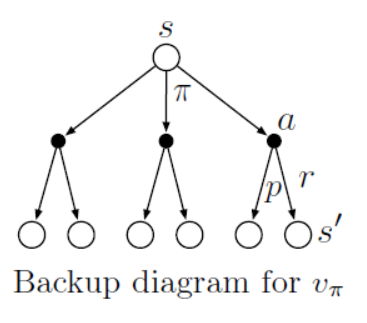
\includegraphics[width=0.4\textwidth]{f3-1-2}
                \caption{值方程的后向传播图}
                \label{f3_1_2}
            \end{figure}
            上图展示了一个起始状态如何分支达到其后续状态的路径,图中空心圆代表状态,而实心圆代表行动。从根节点的起始状态$s$,Agent可以依据策略$\pi$来确定一个行动(也可能有部分的随机性),确定行动之后,Environment会依据概率分布$P(s',r|s,a)$反馈一个新状态和奖励。Bellman方程会在所有的路径上依据概率进行平均。它说明了当前状态的值就必须等于折现后的未来状态的值加上这一条路径上的奖励。

            值方程$v_{\pi}$是Bellman方程的一个特殊解。后续章节会展示Bellman方程是很多计算,近似和学习$v_{\pi}$的基础工具。上图被叫做后向传播图,因为该图刻画了增强学习方法中核心的前向及后向操作。这些操作将值信息从后续节点传递到前向节点。我们在整本书中都会使用这种后向图来对算法进行图解。
        \subsection{最优策略和最优值方程}
            解决增强学习问题的核心就在于确定一种策略可以在长期中获得最大的奖励。对于有限MDPs而言,我们可以通过以下方式较精确地定义一个最优的策略:值方程在策略上做了部分排序,策略$\pi$和策略$\pi '$相比,如果前者在各个状态下的期望收益都要高于后者,那么策略$\pi$就优于或者说不差于策略$\pi '$,换言之,$\pi \ge \pi '$在且仅在条件$v_{\pi}(s) \ge v_{\pi}(s),\ s \in \mathcal{S}$。理论上说,至少存在一个策略有优于或者说不差于其他所有的策略,这个策略就被称为\textbf{最优策略}。尽管可能有很多最优策略,但是我们依然统一记为$\pi_*$。这些最优策略有着相同的状态值方程,称之为\textbf{最优状态值方程},记为$v_*$,定义为:
            \begin{equation}
                v_*(s) \dot{=} \operatorname*{max}\limits_{\pi} v_{\pi}(s),\ \ s\in \mathcal{S}
                \label{e3.15}
            \end{equation}
            同时最优策略同时有着相同的\textbf{最优行动-状态对值方程},记为$q_*$,定义如下:
            \begin{equation}
                q_*(s,a) \dot{=} \operatorname*{max}\limits_{\pi} q_{\pi}(s,a),\ \ s\in \mathcal{S},\ \ a \in \mathcal{A}(s)
                \label{e3.16}
            \end{equation}
            对于行动-状态对$(s,a)$,上述方程给定了在状态$s$和采取行动$a$之后,后续行动的选择遵循最优策略的情形下所能获得的期望回报。因此,我们可以将$q_*$和$v_*$之间的关系记为:
            \begin{equation}
                q_*(s,a) = \mathbb{E}[R_{t+1} + \gamma v_*(S_{t+1})|S_t=s,A_t=a].
                \label{e3.17}
            \end{equation}

            因为$v_*$是某一个策略的值方程,那么它就必须满足由公式\ref{e3.14}所定义的Bellman方程所规定的自洽性条件。但是因为它是最优的值方程,所以$v_*$的自洽性条件可以写成一个不依赖于任何特定策略的特定形式,即$v_*$的Bellman方程或者说是Bellman最优等式。直观上来看,Bellman最优等式说明了在最优策略下,一个状态的值就肯定等于从该状态出发采取最优行动所带来的回报。
            \begin{equation}
                \begin{split}
                    v_*(s) &= \operatorname*{max}\limits_{a\in \mathcal{A}(s)} q_{\pi_*}(s,a) \\
                           &= \operatorname*{max}\limits_{a} \mathbb{E}_{\pi_*}[G_t|S_t=s,A_t=a] \\
                           &= \operatorname*{max}\limits_{a} \mathbb{E}_{\pi_*}[R_{t+1} + \gamma G_{t+1}|S_t=s,A_t=a] \\
                           &= \operatorname*{max}\limits_{a} \mathbb{E}[R_{t+1} + \gamma v_*(S_{t+1})|S_t=s,A_t=a] \\
                           &= \operatorname*{max} \sum_{s',r} P(s',r|s,a) [r + \gamma v_*(s')]
                \end{split}
            \end{equation}
            最后两个等式是$v_*$的Bellman最优等式的两种不同的形式。而$q_*$的Bellman最优等式形式为:
            \begin{equation}
                \begin{split}
                    q_*(s,a) &= \mathbb{E} [R_{t+1}+\gamma \operatorname*{max}\limits_{a'}q_*(S_{t+1},a')|S_t=a,A_t=a] \\
                             &= \sum_{s',r} P(s',r| s,a)[r + \gamma \operatorname*{max}\limits_{a'} q_*(s',a')].
                \end{split}
                \label{e3.20}
            \end{equation}
            图\ref{e3.20}中的流程图形象地展示的$v_*$和$q_*$的Bellman最优等式的计算过程。
            \begin{figure}[h]
                \centering
                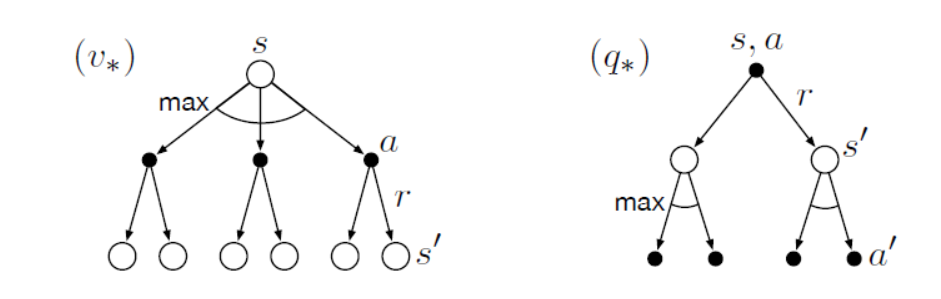
\includegraphics[width=0.6\textwidth]{f3-4}
                \caption{$v_*$和$q_*$的Bellman最优等式的计算过程}
                \label{f3_4}
            \end{figure}

            对于有限MDPS,公式\ref{e3.19}对应的$v_*$的Bellman最优等式是有一个唯一解的。实际上Bellman最优等式是一组方程,每一个状态对应着一个方程,就形成了有$n$个未知数的$n$个方程。如果一个Environment的动态转换概率是已知的,那么原则上讲,使用任何一种求解非线性等式系统的方法都可以求解出$v_*$对应的Bellman最优等式组的解。同样,也可以求解出$q_*$对应的Bellman最优等式组。

            如果能够知道$v_*$,那么最优策略的确定就会非常简单。对于某一个具体状态$s$,依据Bellman最优等式,可能有多个行动可以最大化回报。只要一个策略只给这类行动赋予非零的选中概率,那么它就是最优策略。这可以看作是一步搜索。如果已知最优的值方程$v_*$,那么在一步搜索中奖励最高的行动就是最优行动,换言之,基于最优状态值方程$v_*$的完全贪心搜索策略就是最优的策略。术语贪心在计算机领域指的是在备择选项中选择那些具有即刻最优效果的选项,而不必考虑这些选项可能会造成对未来更优选项的阻碍。更进一步,它刻画的是那些只基于短期序列来进行决策的策略。$v_*$的核心作用在于基于它,一个短视的,贪心的策略和一个长期的,追求全局最优的策略是等价的。通过$v_*$,最优的长期期望收益可以被准确的分配到各个局部的即刻的状态当中,因此,只看一步的搜索策略就可以产生长期最优的策略。

            基于$q_*$来确定最优行动更加简单。有了$q_*$之后,Agent甚至都不需要进行“一步式”的搜索:对于任何状态$s$,根据$q_*(s,a)$可以很快的确定最大的行动,因为这一函数值已经缓存了所有的“一步式”搜索的结果。这一函数值通过局部信息就体现了该行动的长期回报。因此,确定状态-行动对的值函数方程虽然代价比较高,但是基于这个函数就可以做成行动的决策,而不再依赖于任何的后续可能行动以及环境的状态转移特性。

            显式的解决Bellman最优等式方程提供了寻找最优策略的方法,进而解决了增强学习问题。但是这一方法在实际应用中不实用。它本质上就是穷举法,找到所有可能的选项,计算相应的发生概率。这一方法至少依赖于以下三个在实际工作中不太成立的假设:(1)我们确实知道Environment的状态转移矩阵;(2)我们有足够大的计算能力来穷举所有的可能情况;(3)潜在物理过程确实具有马尔科夫性。对于所感兴趣的任务而言,这三个假设基本上不可能同时成立。在国际象棋中,尽管第一条和第三条假设是成立的,但是计算能力去无法完成这一工作,因为有超过$10^20$不同的状态,以目前计算机的计算能力,需要耗费数千年的时间。在增强学习中,大部分时候不得不接受近似结果。

            很多不同的决策方法都可以被视为Bellman最优方程的近似求解。启发式搜索方法可以看做是公式\ref{e3.19}的右侧进行多次展开,构成一颗概率树,然后使用经验估计方法对叶节点位置的$v_*$进行估计。动态规划的方法更接近Bellman最优化方程方法。很多增强学习方法可以被视为使用经验状态转移矩阵来取代真实状态转移矩阵来求解Bellman最优方程。后续章节我们会讨论大量的这一类方法。

        \subsection{最优化和近似}
            目前已经定义了最优值函数和最优策略。当然,掌握了最优策略的Agent可以表现很好,但是实际上这很少出现。对于我们所感兴趣的问题,想要获得最优的策略,就得耗费无限大的计算能力。最优化这一概念在本书中的作用主要是对各个算法的理论性质进行分析,但是实际使用中不得不做很多近似操作。有些问题可能Environment的状态转移特性以及满足马尔科夫性,但是所能调用的计算能力有限。同时,由于状态和行动的组合数量也是巨大的,所以如果遍历所有可能组合的话对存储的压力也是很大的。

            当前关于增强学习的框架致使我们必须接受近似处理,同时,这也促使我们发现了很多有效的近似方法。比如,在近似最优行为中,有一些状态是Agent极少会碰到的,在这些状态上选择一些次优行动,对于总体的回报影响很小。比如在国际象棋机器人中即便它在一些罕见棋盘状态下下棋的水平很低也不影响其在总体上取胜。增强学习的在线学习特性促使其可以通过将主要精力放在经常出现的状态上进行学习而忽略罕见状态来对最优状态进行近似。这是区分增强学习和其他对MDPs过程近似方法的重要特征。

        \subsection{总结}
            接下来对本章学习的增强学习问题的主要特征进行总结。增强学习是关于如何通过行为间交互进行学习以达成目标的方法。它们之间交互的特征定义了一个特殊的任务:由\textbf{Agent}来做出\textbf{行动},\textbf{状态}是采取何种行动的依据,而\textbf{奖励}是评估行动选择是否正确的标准。任何Agent可以完全感知并完全控制的状态称为Agent的\textbf{内部元素},除此之外的元素称之为Agent的外部元素,也就是\textbf{Environment}。\textbf{策略}是Agent基于状态来选择行动的函数。Agent的\textbf{目标}在长期中获得最大的奖励总和。

            依据以上的增强学习设定,如果其状态转移概率是固定的,那么这就是一个马尔科夫过程。而所谓的有限马尔科夫过程指的是状态空间和行动空间都是有限的。目前大部分方法都局限在有限马尔科夫过程上,不过思想具有一定的推广性。

            \textbf{回报}是未来奖励的一个函数,Agent的目标是获得其最大值。根据任务的不同和是否需要考虑折现的问题,这一函数的定义有很大的不同。无折现的形式适用于回合制任务,而有折现的形式适用于持续型任务,不过本章中我们通过定义自吸收状态来将两种不同形式的回报规范为同一形式。

            一个策略对应的\textbf{值方程}是定义在状态空间或者是状态-行动空间上的能返回从该空间点开始所可以获得的最高收益。最优值方程对应的策略称为最优策略。尽管对于一个给定的GDP而言,其最优值方程是唯一的,但可能有多个不同的最优策略。Bellman最优等式是一种最优值方程必须满足的自洽性条件,求解该方程之后就可以获得最优的值方程,以及最优的策略。

            依据先验知识的多少,增强学习可以被表述为不同的形式。在完全知识的情况下,Agent具有环境动态性的全部信息。如果环境满足MDP条件,那么这么环境的模型就有完全的四参数动态方程$p$构成。如果不具备完全的信息,那么一个完备的对环境的建模就是不可行的。

            即便Agent所处的Environment可能是完全清楚且稳定的,那么对值方程进行精确求解所需要计算力和存储也是无法满足的。一个定义良好的最优化可以将本书所要研究的学习方法组织起来,并提供一种可以对比不同学习算法理论性质的方法。本书真正关心的是哪一些情况下增强学习的最优解是无法获得的,只能进行某种程度的近似。

    \section{动态规划}
        术语动态规划指的是一组在给定完全的环境动态特征的条件下可以被用来计算最优策略的算法。传统的DP算法在增强学习中用途不大,一方面是因为它对于完全已知环境的动态特征这个假设很难成立,二方面其计算量非常地大。但是这些方法具有很重要的理论意义。动态规划是理解本书后续算法的必要基础。实际上,后续的那一些算法就是尝试在较少的计算量和非完备信息假设下来实现和动态规划同样的效果。

        通常假设环境是有限MDP,也就是说,假设它的状态,行动,和奖励的集合都是有限的,而且它的动态特性由概率分布$P(s',r|s,a)$来决定。尽管DP方法可以应用与连续状态空间和行动的问题,但是精确解只在某一些特殊情况可以求出。求解连续状态空间和行动空间问题近似解的一般方法就是将状态空间和行动空间离散化,然后使用有限DP方法。第九章讨论的方法适用于连续问题,是DP方法的一种重要拓展。

        DP方法和增强学习方法的关键思想是使用值方程来组织和结构化搜索最优策略的方法。本章我们会讨论DP方法是如何计算值方程的,正如在第三章所说的,一旦计算出满足Bellman最优方程的最优的值方程$v_*,q_*$就可以很容易的得到最优的策略。DP算法本质上就是将Bellman等式转换成一个可以逐步逼近最优值方程的更新方程。

        \subsection{策略估计(预测)}
            首先我们考虑如何计算对于任何策略$\pi$的状态值方程$v_{\pi}$。这在DP算法方面的论文中被称为策略估计问题。我们也将这种方法称为预测问题。根据第三章有,对于任何的$s\in \mathcal{S}$:
            \begin{equation}
                \begin{split}
                    v_{\pi}(s) &\dot{=} \mathbb{E}_{\pi}[G_t|S_t=s] \\
                               &= \mathbb{E}_{\pi}[R_{t+1} + \gamma G_{t+1}| S_t=s] \\
                               &= \mathbb{E}_{\pi}[R_{t+1} + \gamma v_{\pi}(S_{t+1})| S_t=s] \\
                               &= \sum_a \pi(a|s) \sum_{s',r} P(s',r|s,a)[r + \gamma v_{\pi}(s')]
                \end{split}
                \label{e4.4}
            \end{equation}
            其中$\pi(a|s)$指的是基于策略$\pi$处于状态$s$时采取行动$a$的概率,期望收益下的角标$\pi$代表着该收益是基于策略$\pi$的。只要$\gamma<1$或者在策略$\pi$下从任何状态都可以到达最终状态,那么$v_{\pi}$就具有存在性和唯一性。

            如果环境的动态特性是完全可知的,那么公式\ref{e4.4}是建立在$\mathcal{S}$空间上的线性联立方程组。原则上,求解它就是需要冗长单调的计算。不过在本章,我们会使用一种迭代的方式进行求解。假设有一组建立在状态空间上的近似函数$v_0,v_1,v_2,\cdots,v_n$,其初始值的随机选择的(当然除了最终节点之外),其后所有的迭代解可以利用公式\ref{e4.4}(Bellman方程)来得到:
            \begin{equation}
                \begin{split}
                    v_{k+1}(s) &\dot{=} \mathbb{E}_{\pi} [R_{t+1} +\gamma v_k(S_{t+1})| S_t=s] \\
                               &= \sum_a \pi(a|s) \sum_{s',r} P(s',r|s,a)[r + \gamma v_k(s')]
                \end{split}
                \label{e4.5}
            \end{equation}
            对于任何状态$s\in \mathcal{S}$上式均成立。显然,$v_k=v_{\pi}$时更新就不在发生变化了,因为在这种情况下Bellman等式已经成立。实际上,只要$v_{\pi}$存在,那么随着$k\leftarrow \infty$,序列$\{v_k\}$一定会收敛到$v_{\pi}$上。这一算法称为递归式的策略评估方法。

            为了基于$v_k$推导出$v_{k+1}$,递归式策略评估方法在每一个状态$s$上反复执行同样的操作:它将状态$s$的旧值用基于其后续状态的旧值所计算出来的新值来替换,只需要依赖后续一步的状态。我们称这种操作称为期望值更新。迭代式策略评估的每一个轮次会更新所有状态的值以生成新的对值方程的估计结果$v_{k+1}$。有几种不同的期望值更新方法,取决于是状态还是状态-行动对的值在更新,以及后续状态估计值组合的准确方式。在DP算法中所进行的所有的更新操作称之为期望化操作,因为它是基于所有后续可能状态的期望值来计算出来的,而不是后验状态的一个样本。

            为了写一个顺序计算程序来实现公式\ref{e4.5}所示的迭代策略估计,你就需要用到两个数组,第一个数组来存储旧值$v_k(s)$,第二个数组来存放新值$v_{k+1}(s)$。基于这两个数组,新值可以依次从旧值中计算出来,而同时旧值不发生改变。当然也可以使用一个数组,这样的话每次产生新值都覆盖原来的值,而后续计算的新值就会部分依赖于提前产生的新值。这种原地变换算法同样会收敛到$v_{\pi}$,而且收敛速度还要比使用两个数组的方法要快,因为新值一产生就被使用了。我们可以将更新视为是在状态空间中的游走,在原地替换算法中,状态点的更新顺序对于序列的收敛速度是有显著影响的。本书提到的DP算法基本上就是指的原地替换方法。

            完全版本的迭代策略估计(原地替换)算法的伪代码如下:
            \begin{enumerate}
                \item 给定待估计的策略$\pi$
                \item 很小的参数$\theta > 0$,控制估计结果的准确性
                \item 随机设定各个状态$s\in \mathcal{S}$的初始值$V(s)$,只有最终状态$V(terminal)=0$
                \item 循环执行以下代码,直到触发终止条件:
                \begin{enumerate}
                    \item $\Delta \leftarrow 0$
                    \item 依次对各个状态执行以下操作
                    \begin{enumerate}
                        \item $v \leftarrow V(s)$
                        \item $V(s)\leftarrow \sum_a \pi(a|s) \sum_{s',r} P(s',r|s,a)[r + \gamma V(s')]$
                        \item $\Delta \leftarrow max(\Delta,|v-V(s)|)$
                    \end{enumerate}
                \end{enumerate}
            \end{enumerate}

        \subsection{策略改进}
            对某个策略的值方程进行计算的目的是为了搜寻更好的策略。假设我们对任何一个确定性的策略$\pi$的值方程$v_{\pi}$已经了解,那么对于任何状态$s$,我们想知道是否有必要更改策略来确定一个新的行动$a\ne \pi(s)$,同样也想知道更改策略之后总回报是上升还是下降了。解决该问题的一种方法是在状态$s$的基础上选择行动$a$,而之后的行动仍然坚持策略$\pi$,那么这一举动对应的值方程为
            \begin{equation}
                \begin{split}
                    q_{\pi}(s,a) &\dot{=} \mathbb{E}[R_{t+1} + \gamma v_{\pi}(S_{t+1})| S_t = s,A_t = a] \\
                    &= \sum_{s',r} P(s',r|s,a) [r + \gamma v_{\pi}(s')].
                \end{split}
                \label{e4.6}
            \end{equation}
            基于上述公式我们就可以判断出新值与$v_{\pi}$的大小。如果$q_{\pi}(s,a)$比较大,那么在状态$s$时就选择行动$a$,而之后的行动还依赖策略$\pi$来决定行动,那么回报就要高于策略$\pi$的回报,进而就产生了一个新策略。

            上面这个例子是策略改进理论的一个案例。记$\pi$和$\pi '$为两个确定性策略,对于任何的状态$s \in \mathcal{S}$,有:
            \begin{equation}
                q_{\pi} (s,\pi '(s)) \ge v_{\pi}(s)
                \label{e4.7}
            \end{equation}
            那么就可以说策略$\pi '$就要优于策略$\pi$,也就是说策略$\pi '$的总体回报要大于策略$\pi$,
            \begin{equation}
                v_{\pi '}(s) \ge v_{\pi}(s)
                \label{e4.8}
            \end{equation}
            更进一步的,如果公式\ref{e4.7}中有任何一个状态不等式严格成立,那么公式\ref{e4.8}中对应的不等式也是严格成立的。显然公式\ref{e4.7}在各个状态$s$均成立,所以,如果$q_{\pi}(s,a) > v_{\pi}(s)$,那么更改之后的策略就要优于策略$\pi$。

            截止,本章已经说明了在给定策略和值方程的基础上,我们可以很容易的估计策略在单个状态点上作出更改之后对于总回报的影响。自然而然,我们就想是不是可以把所有的状态对应的所有的可能行动都测试一遍,然后根据$q_{\pi}(s,a)$来选择最优的行动。换言之,确定一个新的贪心策略$\pi '$,有:
            \begin{equation}
                \begin{split}
                    \pi '(s) &\dot{=} \operatorname*{argmax}\limits_a q_{\pi}(s,a) \\
                             &= \operatorname*{argmax}\limits_{a} \mathbb{E}[R_{t+1} + \gamma v_{\pi}(S_{t+1})|S_t=s,A_t = a] \\
                             &= \operatorname*{argmax}\limits_{a} \sum_{s',r} P(s',r|s,a) [r+\gamma v_{\pi}(s')]
                \end{split}
                \label{e4.9}
            \end{equation}
            这一贪心策略采取了基于值方程$v_{\pi}$求得的短期最优行动,从构造方程来看,这一贪心策略满足公式\ref{e4.7}(策略改进理论)的条件,那么就可以确定这一贪心策略至少不差于原来的策略。基于值方程上的贪心方法改进原有的策略来构造新策略的方法,叫做策略改进方法(Policy Improvement)。

            假设这个新的贪心策略$\pi '$,是和原来的策略一样好,即$v_{\pi '} = v_{\pi}$,所以根据公式\ref{e4.9}对于所有的状态$s\in \mathcal{S}$有:
            \begin{equation}
                \begin{split}
                    v_{\pi '}(s) &= \operatorname*{max}\limits_{a} \mathbb{E}[R_{t+1} + \gamma v_{\pi '}(S_{t+1})|S_t=s,A_t=a] \\
                                 &= \operatorname*{max}\limits_{a} \sum_{s',r}P(s',r|s,a)[r + \gamma v_{\pi '}(s')].
                \end{split}
            \end{equation}
            但是这个结果和公式\ref{e4.1}(Bellman最优等式)是相同的。因此$v_{\pi '}$就是$v_{*}$,或者说$v_{\pi}$和$v_{\pi '}$都是最优策略。策略改进方法总是可以给出被初始策略更好的策略,除非说原始策略就已经是最优策略了。

        \subsection{策略迭代}
            只要有一个策略$\pi$,那么在环境完全可知的情况下,就可以计算出$v_{\pi}$,进而基于这个值方程,就可以推导出更优的$\pi '$,接下来计算$v_{\pi '}$,进一步就是一个更优的策略$\pi ''$。即可以得到一个持续更新策略和值方程的序列:
            \begin{equation}
                \pi_0 \xrightarrow[]{E} v_{\pi_0} \xrightarrow[]{I} \pi_1 \xrightarrow[]{E} v_{\pi_1} \xrightarrow[]{I} \pi_2 \xrightarrow[]{E} \cdots
                \xrightarrow[]{I} \pi_* \xrightarrow[]{E} v_*
            \end{equation}
            其中$\xrightarrow[]{E}$代表策略估计,而$\xrightarrow[]{I}$代表策略改进。每一次策略改进都是严格意义上的改进(除非它已经是最优的了)。因为有限MDP只有有限个策略,那么上述过程一定会在有限的次数内收敛到最优策略和最优值方程。

            这种确定最优策略的方法称为\textbf{策略迭代}(Policy Iteration)。下述的列表描述了整个算法。在每一轮策略评估中,需要进行循环计算,是从之前策略的值方程可以计算的。这样的方式极大的促进了策略评估的收敛方法。

            \begin{enumerate}
                \item \textbf{初始化}:对于任意的状态$s\in \mathcal{S}$,令$V(s)\in \mathbb{R},\pi(s)\in A(s)$
                \item \textbf{策略评估}:循环执行以下代码:
                \begin{enumerate}
                    \item $\Delta\leftarrow 0$
                    \item 对于所有的状态,执行:
                    \begin{enumerate}
                        \item $v \leftarrow V(s)$
                        \item $V(s) \leftarrow \sum_{s',r} P(s',r|s,\pi(s))[r + \gamma V(s')]$
                        \item $\Delta \leftarrow max(\Delta,|v-V(s)|)$
                    \end{enumerate}
                    直到$\Delta < \theta$($\theta$是一个足够小的超参数)
                \end{enumerate}
                \item \textbf{策略改进}:

                    Policy-Stable $\leftarrow$ True

                    对于所有的状态,执行:
                    \begin{enumerate}
                        \item Old-Action $\leftarrow \pi(s)$
                        \item $\pi(s) \leftarrow \operatorname*{argmax}\limits_{a} \sum_{s',r} P(s',r|s,a)[r + \gamma V(s')]$
                        \item 如果Old-Action$\ne \pi(s)$,那么Policy-Stable$\leftarrow False$
                    \end{enumerate}
                    如果Policy-Stable是真的话,那么停止循环,然后当前的策略和值方程就是最优的策略和值方程,否则的话,回到第2步继续循环。
            \end{enumerate}

        \subsection{值循环方法}
            策略循环方法的一个弊端是它的每一次循环中都需要进行策略评估过程,在策略评估的过程中需要多次穷举整个状态空间,这大大拖慢了计算速度。如果策略评估过程是迭代式的,那么只有在一定的限制条件下序列才能完全收敛到$v_{\pi}$。我们是否有必要一定要等到收敛,是否可以提前退出循环?很多案例表明,没有必要到达完全收敛状态,后续的迭代计算对于确定“短期最优行动”意义不大。

            在策略循环计算中的策略评估过程有几种方法可以提前中断循环,不必到达收敛状态。一种最特殊的情况是,策略评估过程中只进行一次循环,这种特例被称为值循环方法。简单来说,就是将“截断”的策略评估过程和“一般”的策略改进过程结合在一起:
            \begin{equation}
                v_{k+1}(s) \dot{=} \operatorname*{max}\limits_{a}\mathbb{E}[R_{t+1} + \gamma v_k(S_{t+1})|S_t=s,A_t=a]
                     = \operatorname*{max}\limits_{a} \sum_{s',r} P(s',r|s,a)[r+\gamma v_k(s')]
                \label{e4.10}
            \end{equation}
            对于任意的$v_0$,序列$\{v_k\}$在$v_*$存在的情况下也会收敛到$v_*$上。

            另一种理解值循环的方法是和Bellman最优方程。原来的Bellman最优方程是一个判断性条件,即某状态的值等于基于各种后续状态期望下的最优行动对应的值,而这里就是将判断性条件变成了更新法则。

            最后,来考虑值循环方法的终止条件。和策略估计方法一样,值循环方法完全收敛到最优策略对应的值方程上需要无限多次循环。在实际应用中,如果值方程的变化在一轮扫描中变化很小,那么就可以停止迭代了。下述列表是值循环方法的伪代码:
            \begin{enumerate}
                \item \textbf{初始化}:精度参数$\theta>0$,$V(terminal)=0$,其他的状态$V(s)$随机设置。
                \item 执行以下循环:
                \begin{enumerate}
                    \item $\Delta \leftarrow 0$
                    \item 遍历所有的状态$s\in \mathcal{S}$:
                    \begin{enumerate}
                        \item $v \leftarrow V(s)$
                        \item $V(s) \leftarrow \operatorname*{max}\limits_{a} \sum_{s',r} P(s',r|s,a)[r + \gamma V(s')]$
                        \item $\Delta \leftarrow \operatorname*{max}(\Delta,|v-V(s)|)$
                    \end{enumerate}
                \end{enumerate}

                 直到$\Delta < \theta$
                \item 基于值方程可以输出最优策略,即
                $$\pi(s) = \operatorname*{argmax}\limits_{a} \sum_{s',r} P(s',r|s,a)[r + \gamma V(s')] $$
            \end{enumerate}

            值循环方法将一个轮次的策略评估和策略改进高效的结合起来。如果在其中插入几个完整的策略评估加上一个轮次的策略改进,那么收敛速度就会大大加快。一般来说,一个完整的“截断的”策略循环方法可以认为是包括多个轮次,其中一些轮次是进行策略评估更新,而有一些是进行值循环更新。因为公式\ref{e4.10}中的最大化操作是值循环更新和策略评估更新的主要区别,上述操作的含义就是在策略评估的部分轮次中加入最大化操作。这里讨论的各种方法在折现有限马尔科夫过程问题下都可以收敛到最优策略上。

        \subsection{异步动态规划}
            目前讨论的DP算法的主要弊端是它需要对有限马尔科夫过程的整个状态空间进行遍历操作。如果状态空间很大的话,那么这一操作要耗费大量的计算。比如在国际象棋中有$10^20$个不同的状态,即便使用最先进的计算机,有需要上千年的时间进行一次遍历。

            异步DP算法是原地替换的迭代式DP算法,其特点是并不对状态空间进行系统性遍历。该方法以任意的次序使用其他碰巧可用的状态来更新某状态的值。也就是说某一个状态在更新一次的情况下,有的状态已经更新好多次了。但是为了能够正确收敛,异步算法还是需要对所有的状态进行更新:在更新到某种程度之后就不得不更新那些没有更新的状态了。异步的DP算法在选择哪一些状态去更新时具有很大的自由度。

            当然避免扫描所有状态并不意味着计算量很少。它只是说算法没有必要单单进行大量的遍历而策略没有一点点改进。我们可以通过选择对效果改进作用最大的状态点去更新来充分利用这种自由度。这样可以促使我们合理的安排更新次序来高效地评估值函数信息。有一些状态的值更新次数可能比其他状态少很多。甚至如果有些状态点和最优行动无关,那么直接跳过一些状态的值更新。第八章会进一步讨论这一问题。

            异步算法也使得计算和实时交互之间的混合更加容易。为了解决一个特定的MDP问题,在Agent执行MDP的过程中同时可以执行一个迭代式DP算法。Agent的经验可以指导DP算法去更新哪一个状态的值。同时DP算法最近一次的值方程估计和最优策略估计又可以指导决策进行。比如说我们可以更新那些Agent所处的当前状态,这促使DP算法的更新集中于Agent当前所处的周围环境状态。这种重点关注方法是增强学习的一个重要内容。

        \subsection{广义策略迭代}
            策略迭代由两个同步的交互的过程构成,一个是基于当前策略去估计值方程,另一个是基于当前的值方程来“贪心”的确定策略。在策略循环中,这两个过程交替进行,但并不是一成不变的。比如在值迭代方法中,只执行策略评估部分这一个迭代过程;在异步DP算法中,策略评估和策略改进方法在更微小的力度上进行。只要上述两个过程持续更新所有状态,那么最终结果就会收敛到最优的值方程和策略上。

            我们使用术语“广义策略迭代(Generalized Policy Iteration,GPI)”来指代策略评估和策略改进轮次进行的这一类方法。几乎所有的增强学习方法可以概述为GPI的形式,也就是说有可识别的策略和值方程,策略基于值方程来确定,而值方程基于策略来确定。一旦策略估计过程和策略改进过程都稳定了,那么值方程和策略都是最优的。这说明Bellman最优方程成立。

            GPI中的策略评估和策略改进方法既相互竞争也相互促进。两者向不同的方向推进,基于当前策略的值方程估计会促使新策略不是值方程的贪心策略,而基于值方程的策略改进过程促使当前的值方程不成立。不过在长期中,这两个过程推向同一个解:最优的值方程和最优的策略。

        \subsection{动态规划的效率}
            DP算法对于大型问题而言可能不具有可行性,但是相对于其他解决MDPs的方法,DP算法效率还是比较高的。如果忽视一些技术上的细节,DP算法的时间复杂度是状态空间和行动空间的多项式级别。即如果$n$和$k$代表状态和行动的数目,那么DP算法所用到的计算次数应该是小于$n$和$k$的某个多项式函数。这样的算法复杂度是要低于对整个策略空间进行遍历的,因为这样的算法的时间复杂度是$k^n$。线性规划方法有时也被用来解决MDPs问题,并且很多情况下它的时间复杂度上界要小于DP方法,但是状态空间稍微大一些,线性规划的运行效率就下降了。对于特别巨大的问题,只有DP方法是可行的。

            DP算法有时被认为面临维度灾难时适用性较差,这里所说的维度灾难是指随着状态变量的增加,状态空间的规模呈指数级上升。状态空间巨大确实会造成很多问题,但是这是源自于问题本身,而不是DP算法的弊端。实际而言,在面临巨大的状态空间时,DP算法相对于遍历搜索和线性规划要高效很多。

            实际上,以目前的计算机水平,DP算法可以解决带有百万个状态的MDP问题。策略迭代和值迭代方法都在被广泛使用,也很难判断哪一个更好。实际使用中,DP算法的收敛速度要比理论上的上界快得多,尤其是当策略或者值方程的初始值设置合理的情况下。

            当状态空间巨大时,异步DP方法更加适用。为了完成一次遍历,同步的方法就要耗费大量的计算和存储。对于一些问题而言,即便这么大的存储和计算是不可行的,但该问题仍然是可解的,因为只有少量的状态是出现在最优解路径上的。异步方法以及其他GPI方法的变体可以解决该问题,速度也比同步方法更快。

    \section{蒙特卡洛方法}
        本章考虑第一种估计值方程和确定最优策略的学习方法。不同于之前的章节,这里我们不需要假设具有完备的环境知识。MC方法只要求有历史数据的经验--从实际交互中获取的状态,行动,奖励的序列样本。从实际经验中学习困难较大,因为不能利用环境特性的先验知识,但依然可以获得最优的策略。从虚拟的数据中学习也是有种有力的方法,尽管这种情况下也是需要有模型的,但这个模型只需要产生样本的状态转移序列而不需要像DP算法那样给出完整的各个潜在后继状态的概率分布。令人意外地是,很多情形下基于潜在分布产生一个样本是非常容易的,但是想要获得该分布的精确数学表达是很困难的。
        
        蒙特卡洛方法是基于期望样本回报来解决增强学习问题的一种方法。为了确保可以获取良好定义的回报,这里我们讨论的MC方法都只是针对于回合制任务。也就是我们假设经验数据可以切分成独立的回合,而且无论选择何种行动,回合一定会结束。只有在一个回合结束后,值方程和策略才改变一次,也就是说MC方法是基于回合之上的改进方法而不是基于行动之上的改进方法。术语“蒙特卡洛”经常用于刻画带有明确随机性的估计问题上,这里我们用它来特指一类基于期望完全回报的方法(相对而言的方法是那些基于部分回报的方法,下一章会讨论)。
        
        MC方法和赌博机方法一样在状态--行动对上对回报进行平均,在行动上对奖励进行平均。主要的区别是,MC方法所解决的问题往往是多元状态,每一个状态都对应着一个赌博机(就像关联性赌博机或者时序依赖型赌博机一样),且这些赌博机之间都是相互关联的。也就是说,在某一状态下采取一个行动所获得的回报依赖于同一回合内后续状态对应的行动选择。因为所有的行动决策都处于学习当中,所以从早期状态上看环境并不是稳定的。
        
        为了处理这种不稳定性,我们采纳广义策略迭代方法的基本思想。在DP算法中我们使用MDP的先验信息来计算值方程,但在MC方法中我们从MDP的平均回报中计算值方程。值方程和相应的策略仍然需要交互来获取到最优结果。和在DP算法中一样,首先考虑预测问题(也就是基于固定的策略$\pi$来计算$v_{\pi}$和$q_{\pi}$然后是策略改进问题,最终是控制问题和最终解。DP算法的这些思路都可以推广到MC方法上,只不过我们只能获得样本数据,而没有完全的环境先验知识。
        
        \subsection{蒙特卡洛预测}
            我们首先考虑在给定策略的前提下使用MC方法估计状态值方程的估计问题。所谓的状态的值方程就是从该状态开始所能获得的回报的期望(折现的累积回报)。一种显而易见的从历史数据中进行估计的方法就是把经历该状态之后的回报做一下平均。随着越来越多的数据,这个平均数就会收敛到期望值上。这一简单的思想是MC方法的基础。
            
            具体而言,当我们想要获取到基于策略$\pi$的状态$s$的值$v_{\pi}(s)$,同时有一些在策略$\pi$下生产的数据,这些数据都经历过状态$s$。在每一个回合中$s$状态出现就称为途径一次$s$。当然,在一个回合中也有可能多次途径状态s。将在一回合内第一次途径状态$s$称为“第一次途径$s$”,基于第一次访问的MC方法估计$v_{\pi}(s)$是指第一次访问$s$之后期望收益,而多次途径MC方法是基于任何一次访问$s$之后的回报。这两种不同的MC方法很相似,但是在理论性质上有很大的不同。第一次访问MC方法(FVMC)已经被广泛研究,是本章主要的研究对象。历次访问MC方法(EVMC)拓展了函数近似方面的功能,会在第9章和第12章讨论。FVMC方法的具体实现如下所示,而EVMC方法大致相同,除了它不需要检测$S_t$在之前是否出现过。
            \begin{enumerate}
                \item 输入:带估计的策略
                \item 初始化:
                \begin{enumerate}
                    \item $V(s)\in \mathbb{E}$随机设定
                    \item $R(s)=[]$
                \end{enumerate}
                \item 迭代执行以下步骤(每次是一个回合):
                \begin{enumerate}
                    \item 根据策略$\pi$生成回合数据:$S_0,A_0,R_1,S_1,A_1,R_2,\cdots,S_{T-1},A_{T-1},R_T$
                    \item $G \leftarrow 0$
                    \item 迭代执行回合中的每一步,$t = T-1,T-2,\cdots,0$:
                    \begin{enumerate}
                        \item $G\leftarrow \gamma G + R_{t+1}$
                        \item 除非$S_t$出现在$S_0,S_1,\cdots,S_{t-1}$:
                            \begin{enumerate}
                                \item 添加$G$在$R(S_t)$中
                                \item $V(S_t) \leftarrow average(R(S_t))$
                            \end{enumerate}
                    \end{enumerate}
                \end{enumerate}
            \end{enumerate}
            随着途径$s$的次数增多,FVMC和EVMC方法都会收敛到$v_{\pi}(s)$。在FVMC方法上,这一点是很容易理解的。在这种情况下每一个回报都是$v_{\pi}(s)$估计值的独立同分布样本,且方差有限。根据大数定律,平均值的序列就会收敛到它们的期望值。每一个平均值都是期望的无偏估计,而估计的标准差会下降到$1/\sqrt{n}$的水平上,其中$n$指的是途径状态$s$的次数。EVMC不太好理解,但是估计值会以二次的速度收敛到$v_{\pi}(s)$。
            
            下面的例子是理解MC方法的一个好办法。
            
            >> 21点赌博问题
            
            我们能否将流程图的思想用于MC方法呢?DP算法的流程图是从根节点逐步按照可能的状态分叉成树状结构,而MC方法的流程图展示的只是某一个具体回合的样本。另外DP算法的流程图一般只展示一次决策过程的分支和奖励。而MC算法的流程图展示的则是一个完整的回合。这一点上的不同反应了两种算法的核心基础不同。
            
            MC方法的另一个重要特点是对每一个状态的估计是独立。每一个状态的估计都不依赖于其他状态的估计结果。具体而言,就是每一个状态的估计的计算量实际上独立于状态的个数。当我们仅需要部分状态的值时,MC方法的这个特点就显得非常重要。可以设计很多从该状态开始的试验,然后做平均,而不必处理其他状态。
        \subsection{行动值方程的MC估计方法}






\end{document}


